\documentclass[twoside]{book}

% Packages required by doxygen
\usepackage{fixltx2e}
\usepackage{calc}
\usepackage{doxygen}
\usepackage[export]{adjustbox} % also loads graphicx
\usepackage{graphicx}
\usepackage[utf8]{inputenc}
\usepackage{makeidx}
\usepackage{multicol}
\usepackage{multirow}
\PassOptionsToPackage{warn}{textcomp}
\usepackage{textcomp}
\usepackage[nointegrals]{wasysym}
\usepackage[table]{xcolor}

% Font selection
\usepackage[T1]{fontenc}
\usepackage[scaled=.90]{helvet}
\usepackage{courier}
\usepackage{amssymb}
\usepackage{sectsty}
\renewcommand{\familydefault}{\sfdefault}
\allsectionsfont{%
  \fontseries{bc}\selectfont%
  \color{darkgray}%
}
\renewcommand{\DoxyLabelFont}{%
  \fontseries{bc}\selectfont%
  \color{darkgray}%
}
\newcommand{\+}{\discretionary{\mbox{\scriptsize$\hookleftarrow$}}{}{}}

% Page & text layout
\usepackage{geometry}
\geometry{%
  a4paper,%
  top=2.5cm,%
  bottom=2.5cm,%
  left=2.5cm,%
  right=2.5cm%
}
\tolerance=750
\hfuzz=15pt
\hbadness=750
\setlength{\emergencystretch}{15pt}
\setlength{\parindent}{0cm}
\setlength{\parskip}{0.2cm}
\makeatletter
\renewcommand{\paragraph}{%
  \@startsection{paragraph}{4}{0ex}{-1.0ex}{1.0ex}{%
    \normalfont\normalsize\bfseries\SS@parafont%
  }%
}
\renewcommand{\subparagraph}{%
  \@startsection{subparagraph}{5}{0ex}{-1.0ex}{1.0ex}{%
    \normalfont\normalsize\bfseries\SS@subparafont%
  }%
}
\makeatother

% Headers & footers
\usepackage{fancyhdr}
\pagestyle{fancyplain}
\fancyhead[LE]{\fancyplain{}{\bfseries\thepage}}
\fancyhead[CE]{\fancyplain{}{}}
\fancyhead[RE]{\fancyplain{}{\bfseries\leftmark}}
\fancyhead[LO]{\fancyplain{}{\bfseries\rightmark}}
\fancyhead[CO]{\fancyplain{}{}}
\fancyhead[RO]{\fancyplain{}{\bfseries\thepage}}
\fancyfoot[LE]{\fancyplain{}{}}
\fancyfoot[CE]{\fancyplain{}{}}
\fancyfoot[RE]{\fancyplain{}{\bfseries\scriptsize Generated on Fri Mar 27 2015 22\+:04\+:58 for Tennis Assistant -\/ Computer Vision by Doxygen }}
\fancyfoot[LO]{\fancyplain{}{\bfseries\scriptsize Generated on Fri Mar 27 2015 22\+:04\+:58 for Tennis Assistant -\/ Computer Vision by Doxygen }}
\fancyfoot[CO]{\fancyplain{}{}}
\fancyfoot[RO]{\fancyplain{}{}}
\renewcommand{\footrulewidth}{0.4pt}
\renewcommand{\chaptermark}[1]{%
  \markboth{#1}{}%
}
\renewcommand{\sectionmark}[1]{%
  \markright{\thesection\ #1}%
}

% Indices & bibliography
\usepackage{natbib}
\usepackage[titles]{tocloft}
\setcounter{tocdepth}{3}
\setcounter{secnumdepth}{5}
\makeindex

% Hyperlinks (required, but should be loaded last)
\usepackage{ifpdf}
\ifpdf
  \usepackage[pdftex,pagebackref=true]{hyperref}
\else
  \usepackage[ps2pdf,pagebackref=true]{hyperref}
\fi
\hypersetup{%
  colorlinks=true,%
  linkcolor=blue,%
  citecolor=blue,%
  unicode%
}

% Custom commands
\newcommand{\clearemptydoublepage}{%
  \newpage{\pagestyle{empty}\cleardoublepage}%
}


%===== C O N T E N T S =====

\begin{document}

% Titlepage & ToC
\pagenumbering{roman}
\begin{titlepage}
\vspace*{7cm}
\begin{center}%
{\Large Tennis Assistant -\/ Computer Vision }\\
\vspace*{1cm}
{\large Generated by Doxygen 1.8.9.1}\\
\vspace*{0.5cm}
{\small Fri Mar 27 2015 22:04:58}\\
\end{center}
\end{titlepage}
\clearemptydoublepage
\tableofcontents
\clearemptydoublepage
\pagenumbering{arabic}

%--- Begin generated contents ---
\chapter{Namespace Index}
\section{Packages}
Here are the packages with brief descriptions (if available)\+:\begin{DoxyCompactList}
\item\contentsline{section}{\hyperlink{namespacebasket}{basket} }{\pageref{namespacebasket}}{}
\item\contentsline{section}{\hyperlink{namespacebasket__test}{basket\+\_\+test} }{\pageref{namespacebasket__test}}{}
\item\contentsline{section}{\hyperlink{namespaceexperiment}{experiment} }{\pageref{namespaceexperiment}}{}
\item\contentsline{section}{\hyperlink{namespaceimage__support}{image\+\_\+support} }{\pageref{namespaceimage__support}}{}
\item\contentsline{section}{\hyperlink{namespaceparticlefilter}{particlefilter} }{\pageref{namespaceparticlefilter}}{}
\item\contentsline{section}{\hyperlink{namespaceprquadtree}{prquadtree} }{\pageref{namespaceprquadtree}}{}
\item\contentsline{section}{\hyperlink{namespaceprquadtree__test}{prquadtree\+\_\+test} }{\pageref{namespaceprquadtree__test}}{}
\item\contentsline{section}{\hyperlink{namespaceprquadtree__test__example}{prquadtree\+\_\+test\+\_\+example} }{\pageref{namespaceprquadtree__test__example}}{}
\item\contentsline{section}{\hyperlink{namespacetennis__ball}{tennis\+\_\+ball} }{\pageref{namespacetennis__ball}}{}
\item\contentsline{section}{\hyperlink{namespacetennis__ball__test}{tennis\+\_\+ball\+\_\+test} }{\pageref{namespacetennis__ball__test}}{}
\end{DoxyCompactList}

\chapter{Hierarchical Index}
\section{Class Hierarchy}
This inheritance list is sorted roughly, but not completely, alphabetically\+:\begin{DoxyCompactList}
\item \contentsline{section}{prquadtree.\+Box}{\pageref{classprquadtree_1_1Box}}{}
\item \contentsline{section}{particlefilter.\+Particle\+Filter}{\pageref{classparticlefilter_1_1ParticleFilter}}{}
\item \contentsline{section}{prquadtree.\+Point}{\pageref{classprquadtree_1_1Point}}{}
\begin{DoxyCompactList}
\item \contentsline{section}{prquadtree.\+Particle}{\pageref{classprquadtree_1_1Particle}}{}
\end{DoxyCompactList}
\item \contentsline{section}{prquadtree.\+P\+R\+Quad\+Tree}{\pageref{classprquadtree_1_1PRQuadTree}}{}
\item Test\+Case\begin{DoxyCompactList}
\item \contentsline{section}{prquadtree\+\_\+test.\+Test\+Box}{\pageref{classprquadtree__test_1_1TestBox}}{}
\item \contentsline{section}{prquadtree\+\_\+test.\+Test\+Particle}{\pageref{classprquadtree__test_1_1TestParticle}}{}
\item \contentsline{section}{prquadtree\+\_\+test.\+Test\+Point}{\pageref{classprquadtree__test_1_1TestPoint}}{}
\item \contentsline{section}{prquadtree\+\_\+test.\+Test\+Pr\+Quad\+Tree}{\pageref{classprquadtree__test_1_1TestPrQuadTree}}{}
\end{DoxyCompactList}
\end{DoxyCompactList}

\chapter{Class Index}
\section{Class List}
Here are the classes, structs, unions and interfaces with brief descriptions\+:\begin{DoxyCompactList}
\item\contentsline{section}{\hyperlink{classprquadtree_1_1Box}{prquadtree.\+Box} \\*Class defining a square on the coordinate system via a center point and half of square width }{\pageref{classprquadtree_1_1Box}}{}
\item\contentsline{section}{\hyperlink{classprquadtree_1_1Particle}{prquadtree.\+Particle} \\*Represents particle point }{\pageref{classprquadtree_1_1Particle}}{}
\item\contentsline{section}{\hyperlink{classparticlefilter_1_1ParticleFilter}{particlefilter.\+Particle\+Filter} }{\pageref{classparticlefilter_1_1ParticleFilter}}{}
\item\contentsline{section}{\hyperlink{classprquadtree_1_1Point}{prquadtree.\+Point} \\*Represents an (x,y) coordinate point on a grid }{\pageref{classprquadtree_1_1Point}}{}
\item\contentsline{section}{\hyperlink{classprquadtree_1_1PRQuadTree}{prquadtree.\+P\+R\+Quad\+Tree} \\*Class representing a \hyperlink{classprquadtree_1_1Point}{Point} Range Quadtree }{\pageref{classprquadtree_1_1PRQuadTree}}{}
\item\contentsline{section}{\hyperlink{classprquadtree__test_1_1TestBox}{prquadtree\+\_\+test.\+Test\+Box} }{\pageref{classprquadtree__test_1_1TestBox}}{}
\item\contentsline{section}{\hyperlink{classprquadtree__test_1_1TestParticle}{prquadtree\+\_\+test.\+Test\+Particle} }{\pageref{classprquadtree__test_1_1TestParticle}}{}
\item\contentsline{section}{\hyperlink{classprquadtree__test_1_1TestPoint}{prquadtree\+\_\+test.\+Test\+Point} }{\pageref{classprquadtree__test_1_1TestPoint}}{}
\item\contentsline{section}{\hyperlink{classprquadtree__test_1_1TestPrQuadTree}{prquadtree\+\_\+test.\+Test\+Pr\+Quad\+Tree} }{\pageref{classprquadtree__test_1_1TestPrQuadTree}}{}
\end{DoxyCompactList}

\chapter{File Index}
\section{File List}
Here is a list of all files with brief descriptions\+:\begin{DoxyCompactList}
\item\contentsline{section}{\hyperlink{basket_8py}{basket.\+py} }{\pageref{basket_8py}}{}
\item\contentsline{section}{\hyperlink{basket__test_8py}{basket\+\_\+test.\+py} }{\pageref{basket__test_8py}}{}
\item\contentsline{section}{\hyperlink{experiment_8py}{experiment.\+py} }{\pageref{experiment_8py}}{}
\item\contentsline{section}{\hyperlink{image__support_8py}{image\+\_\+support.\+py} }{\pageref{image__support_8py}}{}
\item\contentsline{section}{\hyperlink{particlefilter_8py}{particlefilter.\+py} }{\pageref{particlefilter_8py}}{}
\item\contentsline{section}{\hyperlink{prquadtree_8py}{prquadtree.\+py} }{\pageref{prquadtree_8py}}{}
\item\contentsline{section}{\hyperlink{prquadtree__test_8py}{prquadtree\+\_\+test.\+py} }{\pageref{prquadtree__test_8py}}{}
\item\contentsline{section}{\hyperlink{prquadtree__test__example_8py}{prquadtree\+\_\+test\+\_\+example.\+py} }{\pageref{prquadtree__test__example_8py}}{}
\item\contentsline{section}{\hyperlink{tennis__ball_8py}{tennis\+\_\+ball.\+py} }{\pageref{tennis__ball_8py}}{}
\item\contentsline{section}{\hyperlink{tennis__ball__test_8py}{tennis\+\_\+ball\+\_\+test.\+py} }{\pageref{tennis__ball__test_8py}}{}
\item\contentsline{section}{\hyperlink{visual_8h}{visual.\+h} }{\pageref{visual_8h}}{}
\end{DoxyCompactList}

\chapter{Namespace Documentation}
\hypertarget{namespacebasket}{}\section{basket Namespace Reference}
\label{namespacebasket}\index{basket@{basket}}
\subsection*{Functions}
\begin{DoxyCompactItemize}
\item 
def \hyperlink{namespacebasket_a10ccc2b8542cee4a0e124537a4ca7108}{basket\+\_\+image\+\_\+filter} (img)
\item 
def \hyperlink{namespacebasket_a6244ca5fd7cf7706c81e45e270087d17}{is\+\_\+basket\+\_\+middle} (img)
\item 
def \hyperlink{namespacebasket_a0cb50ef447247bf29a40cbdfcd275bc0}{run\+\_\+middle} ()
\item 
def \hyperlink{namespacebasket_a00c6a996da6d264c30c7b6c710cacddc}{run}
\end{DoxyCompactItemize}
\subsection*{Variables}
\begin{DoxyCompactItemize}
\item 
\hyperlink{namespacebasket_ae8e523df739d65470eb5eba16867f329}{particle\+\_\+filter} = None
\item 
int \hyperlink{namespacebasket_a3c352b285b29250f904de2d4ad7fddaa}{image\+\_\+half\+\_\+size} = -\/1
\item 
int \hyperlink{namespacebasket_a3d020674941ec4faf6734391ca082c40}{save\+\_\+count} = 1
\item 
tuple \hyperlink{namespacebasket_aa3007fa12430ca814f5bf5890bb2fb0f}{base\+\_\+filename} = datetime.\+now()
\end{DoxyCompactItemize}


\subsection{Function Documentation}
\hypertarget{namespacebasket_a10ccc2b8542cee4a0e124537a4ca7108}{}\index{basket@{basket}!basket\+\_\+image\+\_\+filter@{basket\+\_\+image\+\_\+filter}}
\index{basket\+\_\+image\+\_\+filter@{basket\+\_\+image\+\_\+filter}!basket@{basket}}
\subsubsection[{basket\+\_\+image\+\_\+filter}]{\setlength{\rightskip}{0pt plus 5cm}def basket.\+basket\+\_\+image\+\_\+filter (
\begin{DoxyParamCaption}
\item[{}]{img}
\end{DoxyParamCaption}
)}\label{namespacebasket_a10ccc2b8542cee4a0e124537a4ca7108}
\begin{DoxyVerb}Image filter which removes colors out of basket color range. (Deprecated)
@param img SimpleCV.Image
@return img SimpleCV.Image The image with filtered colors turned to black
\end{DoxyVerb}
 \hypertarget{namespacebasket_a6244ca5fd7cf7706c81e45e270087d17}{}\index{basket@{basket}!is\+\_\+basket\+\_\+middle@{is\+\_\+basket\+\_\+middle}}
\index{is\+\_\+basket\+\_\+middle@{is\+\_\+basket\+\_\+middle}!basket@{basket}}
\subsubsection[{is\+\_\+basket\+\_\+middle}]{\setlength{\rightskip}{0pt plus 5cm}def basket.\+is\+\_\+basket\+\_\+middle (
\begin{DoxyParamCaption}
\item[{}]{img}
\end{DoxyParamCaption}
)}\label{namespacebasket_a6244ca5fd7cf7706c81e45e270087d17}
\begin{DoxyVerb}Single entry function returning True/False if basket is in the middle of
the screen
\end{DoxyVerb}
 \hypertarget{namespacebasket_a00c6a996da6d264c30c7b6c710cacddc}{}\index{basket@{basket}!run@{run}}
\index{run@{run}!basket@{basket}}
\subsubsection[{run}]{\setlength{\rightskip}{0pt plus 5cm}def basket.\+run (
\begin{DoxyParamCaption}
\item[{}]{best\+Blob\+Callback = {\ttfamily False}}
\end{DoxyParamCaption}
)}\label{namespacebasket_a00c6a996da6d264c30c7b6c710cacddc}
\hypertarget{namespacebasket_a0cb50ef447247bf29a40cbdfcd275bc0}{}\index{basket@{basket}!run\+\_\+middle@{run\+\_\+middle}}
\index{run\+\_\+middle@{run\+\_\+middle}!basket@{basket}}
\subsubsection[{run\+\_\+middle}]{\setlength{\rightskip}{0pt plus 5cm}def basket.\+run\+\_\+middle (
\begin{DoxyParamCaption}
{}
\end{DoxyParamCaption}
)}\label{namespacebasket_a0cb50ef447247bf29a40cbdfcd275bc0}
\begin{DoxyVerb}Runs continuously and prints if the best detected blob is in the middle
\end{DoxyVerb}
 

\subsection{Variable Documentation}
\hypertarget{namespacebasket_aa3007fa12430ca814f5bf5890bb2fb0f}{}\index{basket@{basket}!base\+\_\+filename@{base\+\_\+filename}}
\index{base\+\_\+filename@{base\+\_\+filename}!basket@{basket}}
\subsubsection[{base\+\_\+filename}]{\setlength{\rightskip}{0pt plus 5cm}tuple basket.\+base\+\_\+filename = datetime.\+now()}\label{namespacebasket_aa3007fa12430ca814f5bf5890bb2fb0f}
\hypertarget{namespacebasket_a3c352b285b29250f904de2d4ad7fddaa}{}\index{basket@{basket}!image\+\_\+half\+\_\+size@{image\+\_\+half\+\_\+size}}
\index{image\+\_\+half\+\_\+size@{image\+\_\+half\+\_\+size}!basket@{basket}}
\subsubsection[{image\+\_\+half\+\_\+size}]{\setlength{\rightskip}{0pt plus 5cm}int basket.\+image\+\_\+half\+\_\+size = -\/1}\label{namespacebasket_a3c352b285b29250f904de2d4ad7fddaa}
\hypertarget{namespacebasket_ae8e523df739d65470eb5eba16867f329}{}\index{basket@{basket}!particle\+\_\+filter@{particle\+\_\+filter}}
\index{particle\+\_\+filter@{particle\+\_\+filter}!basket@{basket}}
\subsubsection[{particle\+\_\+filter}]{\setlength{\rightskip}{0pt plus 5cm}basket.\+particle\+\_\+filter = None}\label{namespacebasket_ae8e523df739d65470eb5eba16867f329}
\hypertarget{namespacebasket_a3d020674941ec4faf6734391ca082c40}{}\index{basket@{basket}!save\+\_\+count@{save\+\_\+count}}
\index{save\+\_\+count@{save\+\_\+count}!basket@{basket}}
\subsubsection[{save\+\_\+count}]{\setlength{\rightskip}{0pt plus 5cm}int basket.\+save\+\_\+count = 1}\label{namespacebasket_a3d020674941ec4faf6734391ca082c40}

\section{basket\+\_\+runner Namespace Reference}
\label{namespacebasket__runner}\index{basket\+\_\+runner@{basket\+\_\+runner}}

\hypertarget{namespacebasket__test}{}\section{basket\+\_\+test Namespace Reference}
\label{namespacebasket__test}\index{basket\+\_\+test@{basket\+\_\+test}}
\subsection*{Functions}
\begin{DoxyCompactItemize}
\item 
def \hyperlink{namespacebasket__test_a6684d8ef9727f3f17d5177625d63f05b}{unit\+Test} (actual, expected, name)
\item 
def \hyperlink{namespacebasket__test_a6e9197dadee8f8fbbaef4c0015ba70d0}{basket\+Present} ()
\item 
def \hyperlink{namespacebasket__test_a02ba4e0e23e1661fbf650bfe5024dd5b}{basket\+Missing} ()
\end{DoxyCompactItemize}


\subsection{Function Documentation}
\hypertarget{namespacebasket__test_a02ba4e0e23e1661fbf650bfe5024dd5b}{}\index{basket\+\_\+test@{basket\+\_\+test}!basket\+Missing@{basket\+Missing}}
\index{basket\+Missing@{basket\+Missing}!basket\+\_\+test@{basket\+\_\+test}}
\subsubsection[{basket\+Missing}]{\setlength{\rightskip}{0pt plus 5cm}def basket\+\_\+test.\+basket\+Missing (
\begin{DoxyParamCaption}
{}
\end{DoxyParamCaption}
)}\label{namespacebasket__test_a02ba4e0e23e1661fbf650bfe5024dd5b}
\hypertarget{namespacebasket__test_a6e9197dadee8f8fbbaef4c0015ba70d0}{}\index{basket\+\_\+test@{basket\+\_\+test}!basket\+Present@{basket\+Present}}
\index{basket\+Present@{basket\+Present}!basket\+\_\+test@{basket\+\_\+test}}
\subsubsection[{basket\+Present}]{\setlength{\rightskip}{0pt plus 5cm}def basket\+\_\+test.\+basket\+Present (
\begin{DoxyParamCaption}
{}
\end{DoxyParamCaption}
)}\label{namespacebasket__test_a6e9197dadee8f8fbbaef4c0015ba70d0}
\hypertarget{namespacebasket__test_a6684d8ef9727f3f17d5177625d63f05b}{}\index{basket\+\_\+test@{basket\+\_\+test}!unit\+Test@{unit\+Test}}
\index{unit\+Test@{unit\+Test}!basket\+\_\+test@{basket\+\_\+test}}
\subsubsection[{unit\+Test}]{\setlength{\rightskip}{0pt plus 5cm}def basket\+\_\+test.\+unit\+Test (
\begin{DoxyParamCaption}
\item[{}]{actual, }
\item[{}]{expected, }
\item[{}]{name}
\end{DoxyParamCaption}
)}\label{namespacebasket__test_a6684d8ef9727f3f17d5177625d63f05b}

\hypertarget{namespaceexperiment}{}\section{experiment Namespace Reference}
\label{namespaceexperiment}\index{experiment@{experiment}}
\subsection*{Functions}
\begin{DoxyCompactItemize}
\item 
def \hyperlink{namespaceexperiment_afd7cadc0db62c738ec5313cac9cd03e5}{experiment}
\item 
def \hyperlink{namespaceexperiment_aeac24644877a02c335d201812ba51625}{hard\+\_\+threshold} (img)
\item 
def \hyperlink{namespaceexperiment_afbfd0da7a229ea75fe6eda26e04a344a}{binary\+\_\+mask} (img)
\item 
def \hyperlink{namespaceexperiment_aad51fba16bbd81e9a968249d747958b3}{dilation\+\_\+and\+\_\+blur} (img)
\item 
def \hyperlink{namespaceexperiment_a26994eacbd1a8bf004fc3477c8164daf}{blobs\+\_\+by\+\_\+mask} (img)
\end{DoxyCompactItemize}


\subsection{Detailed Description}
\begin{DoxyVerb}A utility file for testing out computer vision techniques on preset images.
The purpose of this is to avoid using the webcam, and test on consistent test
cases.
\end{DoxyVerb}
 

\subsection{Function Documentation}
\hypertarget{namespaceexperiment_afbfd0da7a229ea75fe6eda26e04a344a}{}\index{experiment@{experiment}!binary\+\_\+mask@{binary\+\_\+mask}}
\index{binary\+\_\+mask@{binary\+\_\+mask}!experiment@{experiment}}
\subsubsection[{binary\+\_\+mask}]{\setlength{\rightskip}{0pt plus 5cm}def experiment.\+binary\+\_\+mask (
\begin{DoxyParamCaption}
\item[{}]{img}
\end{DoxyParamCaption}
)}\label{namespaceexperiment_afbfd0da7a229ea75fe6eda26e04a344a}
\hypertarget{namespaceexperiment_a26994eacbd1a8bf004fc3477c8164daf}{}\index{experiment@{experiment}!blobs\+\_\+by\+\_\+mask@{blobs\+\_\+by\+\_\+mask}}
\index{blobs\+\_\+by\+\_\+mask@{blobs\+\_\+by\+\_\+mask}!experiment@{experiment}}
\subsubsection[{blobs\+\_\+by\+\_\+mask}]{\setlength{\rightskip}{0pt plus 5cm}def experiment.\+blobs\+\_\+by\+\_\+mask (
\begin{DoxyParamCaption}
\item[{}]{img}
\end{DoxyParamCaption}
)}\label{namespaceexperiment_a26994eacbd1a8bf004fc3477c8164daf}
\hypertarget{namespaceexperiment_aad51fba16bbd81e9a968249d747958b3}{}\index{experiment@{experiment}!dilation\+\_\+and\+\_\+blur@{dilation\+\_\+and\+\_\+blur}}
\index{dilation\+\_\+and\+\_\+blur@{dilation\+\_\+and\+\_\+blur}!experiment@{experiment}}
\subsubsection[{dilation\+\_\+and\+\_\+blur}]{\setlength{\rightskip}{0pt plus 5cm}def experiment.\+dilation\+\_\+and\+\_\+blur (
\begin{DoxyParamCaption}
\item[{}]{img}
\end{DoxyParamCaption}
)}\label{namespaceexperiment_aad51fba16bbd81e9a968249d747958b3}
\hypertarget{namespaceexperiment_afd7cadc0db62c738ec5313cac9cd03e5}{}\index{experiment@{experiment}!experiment@{experiment}}
\index{experiment@{experiment}!experiment@{experiment}}
\subsubsection[{experiment}]{\setlength{\rightskip}{0pt plus 5cm}def experiment.\+experiment (
\begin{DoxyParamCaption}
\item[{}]{image\+\_\+function = {\ttfamily None}, }
\item[{}]{blob\+\_\+function = {\ttfamily None}, }
\item[{}]{directory = {\ttfamily \char`\"{}./\char`\"{}}}
\end{DoxyParamCaption}
)}\label{namespaceexperiment_afd7cadc0db62c738ec5313cac9cd03e5}
\hypertarget{namespaceexperiment_aeac24644877a02c335d201812ba51625}{}\index{experiment@{experiment}!hard\+\_\+threshold@{hard\+\_\+threshold}}
\index{hard\+\_\+threshold@{hard\+\_\+threshold}!experiment@{experiment}}
\subsubsection[{hard\+\_\+threshold}]{\setlength{\rightskip}{0pt plus 5cm}def experiment.\+hard\+\_\+threshold (
\begin{DoxyParamCaption}
\item[{}]{img}
\end{DoxyParamCaption}
)}\label{namespaceexperiment_aeac24644877a02c335d201812ba51625}

\section{image\+\_\+support Namespace Reference}
\label{namespaceimage__support}\index{image\+\_\+support@{image\+\_\+support}}
\subsection*{Functions}
\begin{DoxyCompactItemize}
\item 
def \hyperlink{namespaceimage__support_a45e637a8685d23a453229102a4346327}{external\+\_\+init\+\_\+particle\+\_\+filter} (img)
\begin{DoxyCompactList}\small\item\em Initializes particle filter. \end{DoxyCompactList}\item 
def \hyperlink{namespaceimage__support_aff0422e55f0d6119a012115570442c3f}{image\+\_\+hue\+\_\+filter}
\begin{DoxyCompactList}\small\item\em Converts given image to H\+S\+V based on the given color. \end{DoxyCompactList}\item 
def \hyperlink{namespaceimage__support_aaa6d938c26b4ad5878e1bfb6870e749b}{get\+\_\+hue\+\_\+blobs} (img)
\begin{DoxyCompactList}\small\item\em Gets basket blobs after hue distance filtering. \end{DoxyCompactList}\item 
def \hyperlink{namespaceimage__support_a0cebf9b300caec4b9e3f7725204f7f63}{get\+\_\+best\+\_\+blob} (blobs, particle\+\_\+filter)
\begin{DoxyCompactList}\small\item\em Returns the best blob out of the provided set and particle filter. \end{DoxyCompactList}\item 
def \hyperlink{namespaceimage__support_ae76ebc019a04c735f46210bc29e55f76}{is\+\_\+blob\+\_\+in\+\_\+middle\+\_\+helper} (img, blob)
\begin{DoxyCompactList}\small\item\em Determines whether the given blob is in ceter of image. \end{DoxyCompactList}\end{DoxyCompactItemize}


\subsection{Function Documentation}
\index{image\+\_\+support@{image\+\_\+support}!external\+\_\+init\+\_\+particle\+\_\+filter@{external\+\_\+init\+\_\+particle\+\_\+filter}}
\index{external\+\_\+init\+\_\+particle\+\_\+filter@{external\+\_\+init\+\_\+particle\+\_\+filter}!image\+\_\+support@{image\+\_\+support}}
\subsubsection[{external\+\_\+init\+\_\+particle\+\_\+filter}]{\setlength{\rightskip}{0pt plus 5cm}def image\+\_\+support.\+external\+\_\+init\+\_\+particle\+\_\+filter (
\begin{DoxyParamCaption}
\item[{}]{img}
\end{DoxyParamCaption}
)}\label{namespaceimage__support_a45e637a8685d23a453229102a4346327}


Initializes particle filter. 


\begin{DoxyParams}{Parameters}
{\em img} & Simple\+C\+V.\+Image captured image \\
\hline
\end{DoxyParams}
\begin{DoxyReturn}{Returns}
A Particle\+Filter object 
\end{DoxyReturn}
\index{image\+\_\+support@{image\+\_\+support}!get\+\_\+best\+\_\+blob@{get\+\_\+best\+\_\+blob}}
\index{get\+\_\+best\+\_\+blob@{get\+\_\+best\+\_\+blob}!image\+\_\+support@{image\+\_\+support}}
\subsubsection[{get\+\_\+best\+\_\+blob}]{\setlength{\rightskip}{0pt plus 5cm}def image\+\_\+support.\+get\+\_\+best\+\_\+blob (
\begin{DoxyParamCaption}
\item[{}]{blobs, }
\item[{}]{particle\+\_\+filter}
\end{DoxyParamCaption}
)}\label{namespaceimage__support_a0cebf9b300caec4b9e3f7725204f7f63}


Returns the best blob out of the provided set and particle filter. 


\begin{DoxyParams}{Parameters}
{\em blobs} & list of potential H\+S\+V blobs \\
\hline
{\em particle\+\_\+filter} & initialized Particle\+Filter object \\
\hline
\end{DoxyParams}
\begin{DoxyReturn}{Returns}
The largest blob found or None. 
\end{DoxyReturn}
\index{image\+\_\+support@{image\+\_\+support}!get\+\_\+hue\+\_\+blobs@{get\+\_\+hue\+\_\+blobs}}
\index{get\+\_\+hue\+\_\+blobs@{get\+\_\+hue\+\_\+blobs}!image\+\_\+support@{image\+\_\+support}}
\subsubsection[{get\+\_\+hue\+\_\+blobs}]{\setlength{\rightskip}{0pt plus 5cm}def image\+\_\+support.\+get\+\_\+hue\+\_\+blobs (
\begin{DoxyParamCaption}
\item[{}]{img}
\end{DoxyParamCaption}
)}\label{namespaceimage__support_aaa6d938c26b4ad5878e1bfb6870e749b}


Gets basket blobs after hue distance filtering. 


\begin{DoxyParams}{Parameters}
{\em img} & Simple\+C\+V.\+Image captured image. \\
\hline
\end{DoxyParams}
\begin{DoxyReturn}{Returns}
Set of \textquotesingle{}black\textquotesingle{} potential blobs. 
\end{DoxyReturn}
\index{image\+\_\+support@{image\+\_\+support}!image\+\_\+hue\+\_\+filter@{image\+\_\+hue\+\_\+filter}}
\index{image\+\_\+hue\+\_\+filter@{image\+\_\+hue\+\_\+filter}!image\+\_\+support@{image\+\_\+support}}
\subsubsection[{image\+\_\+hue\+\_\+filter}]{\setlength{\rightskip}{0pt plus 5cm}def image\+\_\+support.\+image\+\_\+hue\+\_\+filter (
\begin{DoxyParamCaption}
\item[{}]{img, }
\item[{}]{ball = {\ttfamily True}}
\end{DoxyParamCaption}
)}\label{namespaceimage__support_aff0422e55f0d6119a012115570442c3f}


Converts given image to H\+S\+V based on the given color. 


\begin{DoxyParams}{Parameters}
{\em img} & Simple\+C\+V.\+Image captured image \\
\hline
{\em color} & tuple of R\+G\+B values of singe \textquotesingle{}H\textquotesingle{} value of H\+S\+V \\
\hline
\end{DoxyParams}
\begin{DoxyReturn}{Returns}
H\+S\+V converted image 
\end{DoxyReturn}
\index{image\+\_\+support@{image\+\_\+support}!is\+\_\+blob\+\_\+in\+\_\+middle\+\_\+helper@{is\+\_\+blob\+\_\+in\+\_\+middle\+\_\+helper}}
\index{is\+\_\+blob\+\_\+in\+\_\+middle\+\_\+helper@{is\+\_\+blob\+\_\+in\+\_\+middle\+\_\+helper}!image\+\_\+support@{image\+\_\+support}}
\subsubsection[{is\+\_\+blob\+\_\+in\+\_\+middle\+\_\+helper}]{\setlength{\rightskip}{0pt plus 5cm}def image\+\_\+support.\+is\+\_\+blob\+\_\+in\+\_\+middle\+\_\+helper (
\begin{DoxyParamCaption}
\item[{}]{img, }
\item[{}]{blob}
\end{DoxyParamCaption}
)}\label{namespaceimage__support_ae76ebc019a04c735f46210bc29e55f76}


Determines whether the given blob is in ceter of image. 


\begin{DoxyParams}{Parameters}
{\em img} & Simple\+C\+V.\+Image caputed image \\
\hline
{\em blob} & Simple\+C\+V.\+Blob Blob object \\
\hline
\end{DoxyParams}
\begin{DoxyReturn}{Returns}
True if blob in middle of image, false otherwise. 
\end{DoxyReturn}

\section{particlefilter Namespace Reference}
\label{namespaceparticlefilter}\index{particlefilter@{particlefilter}}
\subsection*{Classes}
\begin{DoxyCompactItemize}
\item 
class \hyperlink{classparticlefilter_1_1ParticleFilter}{Particle\+Filter}
\end{DoxyCompactItemize}

\section{prquadtree Namespace Reference}
\label{namespaceprquadtree}\index{prquadtree@{prquadtree}}
\subsection*{Classes}
\begin{DoxyCompactItemize}
\item 
class \hyperlink{classprquadtree_1_1Box}{Box}
\begin{DoxyCompactList}\small\item\em Class defining a square on the coordinate system via a center point and half of square width. \end{DoxyCompactList}\item 
class \hyperlink{classprquadtree_1_1Particle}{Particle}
\begin{DoxyCompactList}\small\item\em Represents particle point. \end{DoxyCompactList}\item 
class \hyperlink{classprquadtree_1_1Point}{Point}
\begin{DoxyCompactList}\small\item\em Represents an (x,y) coordinate point on a grid. \end{DoxyCompactList}\item 
class \hyperlink{classprquadtree_1_1PRQuadTree}{P\+R\+Quad\+Tree}
\begin{DoxyCompactList}\small\item\em Class representing a \hyperlink{classprquadtree_1_1Point}{Point} Range Quadtree. \end{DoxyCompactList}\end{DoxyCompactItemize}


\subsection{Detailed Description}
\begin{DoxyVerb}Implementation of a Point Range Quadtree.

Author: Pawel Szczurko
\end{DoxyVerb}
 
\section{prquadtree\+\_\+test Namespace Reference}
\label{namespaceprquadtree__test}\index{prquadtree\+\_\+test@{prquadtree\+\_\+test}}
\subsection*{Classes}
\begin{DoxyCompactItemize}
\item 
class \hyperlink{classprquadtree__test_1_1TestBox}{Test\+Box}
\item 
class \hyperlink{classprquadtree__test_1_1TestParticle}{Test\+Particle}
\item 
class \hyperlink{classprquadtree__test_1_1TestPoint}{Test\+Point}
\item 
class \hyperlink{classprquadtree__test_1_1TestPrQuadTree}{Test\+Pr\+Quad\+Tree}
\end{DoxyCompactItemize}

\section{prquadtree\+\_\+test\+\_\+example Namespace Reference}
\label{namespaceprquadtree__test__example}\index{prquadtree\+\_\+test\+\_\+example@{prquadtree\+\_\+test\+\_\+example}}
\subsection*{Variables}
\begin{DoxyCompactItemize}
\item 
tuple \hyperlink{namespaceprquadtree__test__example_a430c6e4c1960cb0326d40a60be817d65}{b} = \hyperlink{classprquadtree_1_1Box}{Box}(\hyperlink{classprquadtree_1_1Point}{Point}(5,5), 50)
\item 
tuple \hyperlink{namespaceprquadtree__test__example_a6c76891a5f566a70e8ab91c9946be5a2}{b2} = \hyperlink{classprquadtree_1_1Box}{Box}(\hyperlink{classprquadtree_1_1Point}{Point}(50,50), 50)
\item 
tuple \hyperlink{namespaceprquadtree__test__example_a92699a8bb92121b0ffdac66d511f3359}{qt} = \hyperlink{classprquadtree_1_1PRQuadTree}{P\+R\+Quad\+Tree}(\hyperlink{namespaceprquadtree__test__example_a6c76891a5f566a70e8ab91c9946be5a2}{b2})
\item 
tuple \hyperlink{namespaceprquadtree__test__example_ab0091dbc0243fa027e0bc7025d8ea3ad}{pt} = \hyperlink{classprquadtree_1_1Point}{Point}(2,2)
\item 
tuple \hyperlink{namespaceprquadtree__test__example_a2024920106d8770dc2cfa9da1e4fe410}{nearby} = qt.\+query\+\_\+k\+\_\+nearest(\hyperlink{namespaceprquadtree__test__example_ab0091dbc0243fa027e0bc7025d8ea3ad}{pt}, 20)
\item 
int \hyperlink{namespaceprquadtree__test__example_a51f7199631c374c21ed3dada86cc3766}{c} = 1
\end{DoxyCompactItemize}


\subsection{Detailed Description}
\begin{DoxyVerb}File testing the capabilities of the PRQuadTree.

Author: Pawel Szczurko
\end{DoxyVerb}
 

\subsection{Variable Documentation}
\index{prquadtree\+\_\+test\+\_\+example@{prquadtree\+\_\+test\+\_\+example}!b@{b}}
\index{b@{b}!prquadtree\+\_\+test\+\_\+example@{prquadtree\+\_\+test\+\_\+example}}
\subsubsection[{b}]{\setlength{\rightskip}{0pt plus 5cm}tuple prquadtree\+\_\+test\+\_\+example.\+b = {\bf Box}({\bf Point}(5,5), 50)}\label{namespaceprquadtree__test__example_a430c6e4c1960cb0326d40a60be817d65}
\index{prquadtree\+\_\+test\+\_\+example@{prquadtree\+\_\+test\+\_\+example}!b2@{b2}}
\index{b2@{b2}!prquadtree\+\_\+test\+\_\+example@{prquadtree\+\_\+test\+\_\+example}}
\subsubsection[{b2}]{\setlength{\rightskip}{0pt plus 5cm}tuple prquadtree\+\_\+test\+\_\+example.\+b2 = {\bf Box}({\bf Point}(50,50), 50)}\label{namespaceprquadtree__test__example_a6c76891a5f566a70e8ab91c9946be5a2}
\index{prquadtree\+\_\+test\+\_\+example@{prquadtree\+\_\+test\+\_\+example}!c@{c}}
\index{c@{c}!prquadtree\+\_\+test\+\_\+example@{prquadtree\+\_\+test\+\_\+example}}
\subsubsection[{c}]{\setlength{\rightskip}{0pt plus 5cm}int prquadtree\+\_\+test\+\_\+example.\+c = 1}\label{namespaceprquadtree__test__example_a51f7199631c374c21ed3dada86cc3766}
\index{prquadtree\+\_\+test\+\_\+example@{prquadtree\+\_\+test\+\_\+example}!nearby@{nearby}}
\index{nearby@{nearby}!prquadtree\+\_\+test\+\_\+example@{prquadtree\+\_\+test\+\_\+example}}
\subsubsection[{nearby}]{\setlength{\rightskip}{0pt plus 5cm}tuple prquadtree\+\_\+test\+\_\+example.\+nearby = qt.\+query\+\_\+k\+\_\+nearest({\bf pt}, 20)}\label{namespaceprquadtree__test__example_a2024920106d8770dc2cfa9da1e4fe410}
\index{prquadtree\+\_\+test\+\_\+example@{prquadtree\+\_\+test\+\_\+example}!pt@{pt}}
\index{pt@{pt}!prquadtree\+\_\+test\+\_\+example@{prquadtree\+\_\+test\+\_\+example}}
\subsubsection[{pt}]{\setlength{\rightskip}{0pt plus 5cm}tuple prquadtree\+\_\+test\+\_\+example.\+pt = {\bf Point}(2,2)}\label{namespaceprquadtree__test__example_ab0091dbc0243fa027e0bc7025d8ea3ad}
\index{prquadtree\+\_\+test\+\_\+example@{prquadtree\+\_\+test\+\_\+example}!qt@{qt}}
\index{qt@{qt}!prquadtree\+\_\+test\+\_\+example@{prquadtree\+\_\+test\+\_\+example}}
\subsubsection[{qt}]{\setlength{\rightskip}{0pt plus 5cm}tuple prquadtree\+\_\+test\+\_\+example.\+qt = {\bf P\+R\+Quad\+Tree}({\bf b2})}\label{namespaceprquadtree__test__example_a92699a8bb92121b0ffdac66d511f3359}

\section{tennis\+\_\+ball Namespace Reference}
\label{namespacetennis__ball}\index{tennis\+\_\+ball@{tennis\+\_\+ball}}
\subsection*{Functions}
\begin{DoxyCompactItemize}
\item 
def \hyperlink{namespacetennis__ball_a595850f165f1ae2c78218d580854bfda}{is\+\_\+ball\+\_\+middle} (img)
\begin{DoxyCompactList}\small\item\em Entry point for module which determines whether tennis ball is in the middle of the image. \end{DoxyCompactList}\item 
def \hyperlink{namespacetennis__ball_af2aced0030d28f7b0b98175dd3a3d97c}{run} ()
\begin{DoxyCompactList}\small\item\em Continuously captures image from computer camera and feeds it to the is\+\_\+ball\+\_\+middle method to detect whether tennis ball is in the middle of the screen. \end{DoxyCompactList}\end{DoxyCompactItemize}
\subsection*{Variables}
\begin{DoxyCompactItemize}
\item 
\hyperlink{namespacetennis__ball_aba3913b89ed8c5fae700b6dfbca98f05}{particle\+\_\+filter} = None
\end{DoxyCompactItemize}


\subsection{Detailed Description}
\begin{DoxyVerb}Simple detection of ball using SimpleCV (much easier than OpenCV). The run method
identifies a tennis ball in the camera stream image. 'is_ball_middle' function
can be used to determine whether a ball is horizontally centered based on a specified
threshold.

-Pawel Szczurko
\end{DoxyVerb}
 

\subsection{Function Documentation}
\index{tennis\+\_\+ball@{tennis\+\_\+ball}!is\+\_\+ball\+\_\+middle@{is\+\_\+ball\+\_\+middle}}
\index{is\+\_\+ball\+\_\+middle@{is\+\_\+ball\+\_\+middle}!tennis\+\_\+ball@{tennis\+\_\+ball}}
\subsubsection[{is\+\_\+ball\+\_\+middle}]{\setlength{\rightskip}{0pt plus 5cm}def tennis\+\_\+ball.\+is\+\_\+ball\+\_\+middle (
\begin{DoxyParamCaption}
\item[{}]{img}
\end{DoxyParamCaption}
)}\label{namespacetennis__ball_a595850f165f1ae2c78218d580854bfda}


Entry point for module which determines whether tennis ball is in the middle of the image. 


\begin{DoxyParams}{Parameters}
{\em img} & Simple\+C\+V.\+Image \\
\hline
\end{DoxyParams}
\begin{DoxyReturn}{Returns}
boolean. True if tennis ball is in middle, false otherwise. 
\end{DoxyReturn}
\index{tennis\+\_\+ball@{tennis\+\_\+ball}!run@{run}}
\index{run@{run}!tennis\+\_\+ball@{tennis\+\_\+ball}}
\subsubsection[{run}]{\setlength{\rightskip}{0pt plus 5cm}def tennis\+\_\+ball.\+run (
\begin{DoxyParamCaption}
{}
\end{DoxyParamCaption}
)}\label{namespacetennis__ball_af2aced0030d28f7b0b98175dd3a3d97c}


Continuously captures image from computer camera and feeds it to the is\+\_\+ball\+\_\+middle method to detect whether tennis ball is in the middle of the screen. 



\subsection{Variable Documentation}
\index{tennis\+\_\+ball@{tennis\+\_\+ball}!particle\+\_\+filter@{particle\+\_\+filter}}
\index{particle\+\_\+filter@{particle\+\_\+filter}!tennis\+\_\+ball@{tennis\+\_\+ball}}
\subsubsection[{particle\+\_\+filter}]{\setlength{\rightskip}{0pt plus 5cm}tennis\+\_\+ball.\+particle\+\_\+filter = None}\label{namespacetennis__ball_aba3913b89ed8c5fae700b6dfbca98f05}

\section{tennis\+\_\+ball\+\_\+runner Namespace Reference}
\label{namespacetennis__ball__runner}\index{tennis\+\_\+ball\+\_\+runner@{tennis\+\_\+ball\+\_\+runner}}

\hypertarget{namespacetennis__ball__test}{}\section{tennis\+\_\+ball\+\_\+test Namespace Reference}
\label{namespacetennis__ball__test}\index{tennis\+\_\+ball\+\_\+test@{tennis\+\_\+ball\+\_\+test}}
\subsection*{Functions}
\begin{DoxyCompactItemize}
\item 
def \hyperlink{namespacetennis__ball__test_a377f9e4b2c183f3b84a826938e92b1d3}{unit\+Test} (actual, expected, name)
\item 
def \hyperlink{namespacetennis__ball__test_ae38438bf59080ab5cb67dc008a0e05b5}{ball\+Present} ()
\item 
def \hyperlink{namespacetennis__ball__test_a62d3502cccff6477767acdf8cf20caab}{ball\+Missing} ()
\end{DoxyCompactItemize}


\subsection{Function Documentation}
\hypertarget{namespacetennis__ball__test_a62d3502cccff6477767acdf8cf20caab}{}\index{tennis\+\_\+ball\+\_\+test@{tennis\+\_\+ball\+\_\+test}!ball\+Missing@{ball\+Missing}}
\index{ball\+Missing@{ball\+Missing}!tennis\+\_\+ball\+\_\+test@{tennis\+\_\+ball\+\_\+test}}
\subsubsection[{ball\+Missing}]{\setlength{\rightskip}{0pt plus 5cm}def tennis\+\_\+ball\+\_\+test.\+ball\+Missing (
\begin{DoxyParamCaption}
{}
\end{DoxyParamCaption}
)}\label{namespacetennis__ball__test_a62d3502cccff6477767acdf8cf20caab}
\hypertarget{namespacetennis__ball__test_ae38438bf59080ab5cb67dc008a0e05b5}{}\index{tennis\+\_\+ball\+\_\+test@{tennis\+\_\+ball\+\_\+test}!ball\+Present@{ball\+Present}}
\index{ball\+Present@{ball\+Present}!tennis\+\_\+ball\+\_\+test@{tennis\+\_\+ball\+\_\+test}}
\subsubsection[{ball\+Present}]{\setlength{\rightskip}{0pt plus 5cm}def tennis\+\_\+ball\+\_\+test.\+ball\+Present (
\begin{DoxyParamCaption}
{}
\end{DoxyParamCaption}
)}\label{namespacetennis__ball__test_ae38438bf59080ab5cb67dc008a0e05b5}
\hypertarget{namespacetennis__ball__test_a377f9e4b2c183f3b84a826938e92b1d3}{}\index{tennis\+\_\+ball\+\_\+test@{tennis\+\_\+ball\+\_\+test}!unit\+Test@{unit\+Test}}
\index{unit\+Test@{unit\+Test}!tennis\+\_\+ball\+\_\+test@{tennis\+\_\+ball\+\_\+test}}
\subsubsection[{unit\+Test}]{\setlength{\rightskip}{0pt plus 5cm}def tennis\+\_\+ball\+\_\+test.\+unit\+Test (
\begin{DoxyParamCaption}
\item[{}]{actual, }
\item[{}]{expected, }
\item[{}]{name}
\end{DoxyParamCaption}
)}\label{namespacetennis__ball__test_a377f9e4b2c183f3b84a826938e92b1d3}

\chapter{Class Documentation}
\hypertarget{classprquadtree_1_1Box}{}\section{prquadtree.\+Box Class Reference}
\label{classprquadtree_1_1Box}\index{prquadtree.\+Box@{prquadtree.\+Box}}
\subsection*{Public Member Functions}
\begin{DoxyCompactItemize}
\item 
def \hyperlink{classprquadtree_1_1Box_a0ff4532e81c55a7b41c35e85b0099168}{\+\_\+\+\_\+init\+\_\+\+\_\+} (self, center, half\+\_\+size)
\item 
def \hyperlink{classprquadtree_1_1Box_a3f8878c3fa9a89b786103d31821304df}{contains\+\_\+point} (self, point)
\item 
def \hyperlink{classprquadtree_1_1Box_af8b0a29f1094809b6ae0793077d51648}{intersect} (self, other\+\_\+box)
\end{DoxyCompactItemize}
\subsection*{Public Attributes}
\begin{DoxyCompactItemize}
\item 
\hypertarget{classprquadtree_1_1Box_a97475b97164cac388fc673e08ce2707e}{}{\bfseries center}\label{classprquadtree_1_1Box_a97475b97164cac388fc673e08ce2707e}

\item 
\hypertarget{classprquadtree_1_1Box_ac40b9c6e566a2ca829a2e84e3f741294}{}{\bfseries half\+\_\+size}\label{classprquadtree_1_1Box_ac40b9c6e566a2ca829a2e84e3f741294}

\end{DoxyCompactItemize}


\subsection{Detailed Description}
\begin{DoxyVerb}Class defining a square on the coordinate system via a center point and
half of square width.
\end{DoxyVerb}
 

\subsection{Constructor \& Destructor Documentation}
\hypertarget{classprquadtree_1_1Box_a0ff4532e81c55a7b41c35e85b0099168}{}\index{prquadtree\+::\+Box@{prquadtree\+::\+Box}!\+\_\+\+\_\+init\+\_\+\+\_\+@{\+\_\+\+\_\+init\+\_\+\+\_\+}}
\index{\+\_\+\+\_\+init\+\_\+\+\_\+@{\+\_\+\+\_\+init\+\_\+\+\_\+}!prquadtree\+::\+Box@{prquadtree\+::\+Box}}
\subsubsection[{\+\_\+\+\_\+init\+\_\+\+\_\+}]{\setlength{\rightskip}{0pt plus 5cm}def prquadtree.\+Box.\+\_\+\+\_\+init\+\_\+\+\_\+ (
\begin{DoxyParamCaption}
\item[{}]{self, }
\item[{}]{center, }
\item[{}]{half\+\_\+size}
\end{DoxyParamCaption}
)}\label{classprquadtree_1_1Box_a0ff4532e81c55a7b41c35e85b0099168}
\begin{DoxyVerb}Construct a Box object.

Args:
    center: a Point type specifying the center of the square
    half_size: half the length of the square
\end{DoxyVerb}
 

\subsection{Member Function Documentation}
\hypertarget{classprquadtree_1_1Box_a3f8878c3fa9a89b786103d31821304df}{}\index{prquadtree\+::\+Box@{prquadtree\+::\+Box}!contains\+\_\+point@{contains\+\_\+point}}
\index{contains\+\_\+point@{contains\+\_\+point}!prquadtree\+::\+Box@{prquadtree\+::\+Box}}
\subsubsection[{contains\+\_\+point}]{\setlength{\rightskip}{0pt plus 5cm}def prquadtree.\+Box.\+contains\+\_\+point (
\begin{DoxyParamCaption}
\item[{}]{self, }
\item[{}]{point}
\end{DoxyParamCaption}
)}\label{classprquadtree_1_1Box_a3f8878c3fa9a89b786103d31821304df}
\begin{DoxyVerb}Verifies that the given point is within this square.

Args:
    point: a Point type to check if it's in the square

Returns:
    A boolean indicating whether the point is within the square
\end{DoxyVerb}
 \hypertarget{classprquadtree_1_1Box_af8b0a29f1094809b6ae0793077d51648}{}\index{prquadtree\+::\+Box@{prquadtree\+::\+Box}!intersect@{intersect}}
\index{intersect@{intersect}!prquadtree\+::\+Box@{prquadtree\+::\+Box}}
\subsubsection[{intersect}]{\setlength{\rightskip}{0pt plus 5cm}def prquadtree.\+Box.\+intersect (
\begin{DoxyParamCaption}
\item[{}]{self, }
\item[{}]{other\+\_\+box}
\end{DoxyParamCaption}
)}\label{classprquadtree_1_1Box_af8b0a29f1094809b6ae0793077d51648}
\begin{DoxyVerb}Checks if the provided box/square intersects with this square.

Args:
    other_box: another Box object

Returns:
    A boolean indicating if the two intersect anywhere
\end{DoxyVerb}
 

The documentation for this class was generated from the following file\+:\begin{DoxyCompactItemize}
\item 
prquadtree.\+py\end{DoxyCompactItemize}

\hypertarget{classprquadtree_1_1Particle}{}\section{prquadtree.\+Particle Class Reference}
\label{classprquadtree_1_1Particle}\index{prquadtree.\+Particle@{prquadtree.\+Particle}}
Inheritance diagram for prquadtree.\+Particle\+:\begin{figure}[H]
\begin{center}
\leavevmode
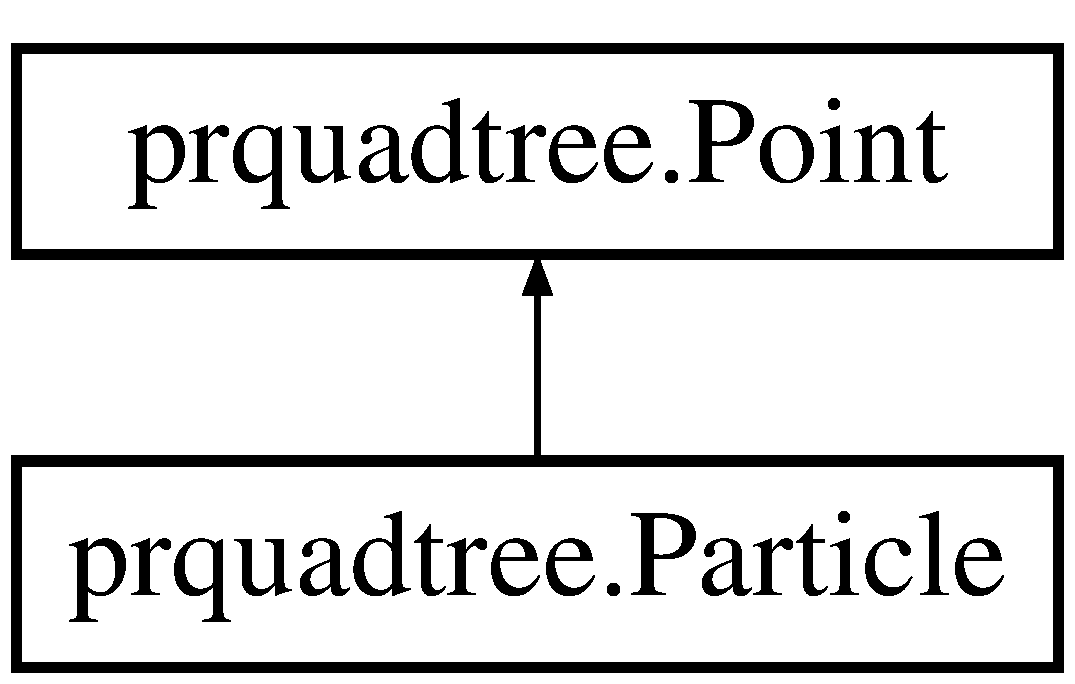
\includegraphics[height=2.000000cm]{classprquadtree_1_1Particle}
\end{center}
\end{figure}
\subsection*{Public Member Functions}
\begin{DoxyCompactItemize}
\item 
def \hyperlink{classprquadtree_1_1Particle_a4508876870d2813145a26fb581ce06f4}{\+\_\+\+\_\+init\+\_\+\+\_\+} (self, \hyperlink{classprquadtree_1_1Particle_a749ee47de3358225c48e7b8d4dc85ded}{x}, \hyperlink{classprquadtree_1_1Particle_ab4bcb8c94d6976d2050749590ad41210}{y})
\end{DoxyCompactItemize}
\subsection*{Public Attributes}
\begin{DoxyCompactItemize}
\item 
\hyperlink{classprquadtree_1_1Particle_a749ee47de3358225c48e7b8d4dc85ded}{x}
\item 
\hyperlink{classprquadtree_1_1Particle_ab4bcb8c94d6976d2050749590ad41210}{y}
\item 
\hyperlink{classprquadtree_1_1Particle_a9fc6fbbd51a3dc21b0dc2531c6c6ff1b}{score}
\end{DoxyCompactItemize}


\subsection{Constructor \& Destructor Documentation}
\hypertarget{classprquadtree_1_1Particle_a4508876870d2813145a26fb581ce06f4}{}\index{prquadtree\+::\+Particle@{prquadtree\+::\+Particle}!\+\_\+\+\_\+init\+\_\+\+\_\+@{\+\_\+\+\_\+init\+\_\+\+\_\+}}
\index{\+\_\+\+\_\+init\+\_\+\+\_\+@{\+\_\+\+\_\+init\+\_\+\+\_\+}!prquadtree\+::\+Particle@{prquadtree\+::\+Particle}}
\subsubsection[{\+\_\+\+\_\+init\+\_\+\+\_\+}]{\setlength{\rightskip}{0pt plus 5cm}def prquadtree.\+Particle.\+\_\+\+\_\+init\+\_\+\+\_\+ (
\begin{DoxyParamCaption}
\item[{}]{self, }
\item[{}]{x, }
\item[{}]{y}
\end{DoxyParamCaption}
)}\label{classprquadtree_1_1Particle_a4508876870d2813145a26fb581ce06f4}


\subsection{Member Data Documentation}
\hypertarget{classprquadtree_1_1Particle_a9fc6fbbd51a3dc21b0dc2531c6c6ff1b}{}\index{prquadtree\+::\+Particle@{prquadtree\+::\+Particle}!score@{score}}
\index{score@{score}!prquadtree\+::\+Particle@{prquadtree\+::\+Particle}}
\subsubsection[{score}]{\setlength{\rightskip}{0pt plus 5cm}prquadtree.\+Particle.\+score}\label{classprquadtree_1_1Particle_a9fc6fbbd51a3dc21b0dc2531c6c6ff1b}
\hypertarget{classprquadtree_1_1Particle_a749ee47de3358225c48e7b8d4dc85ded}{}\index{prquadtree\+::\+Particle@{prquadtree\+::\+Particle}!x@{x}}
\index{x@{x}!prquadtree\+::\+Particle@{prquadtree\+::\+Particle}}
\subsubsection[{x}]{\setlength{\rightskip}{0pt plus 5cm}prquadtree.\+Particle.\+x}\label{classprquadtree_1_1Particle_a749ee47de3358225c48e7b8d4dc85ded}
\hypertarget{classprquadtree_1_1Particle_ab4bcb8c94d6976d2050749590ad41210}{}\index{prquadtree\+::\+Particle@{prquadtree\+::\+Particle}!y@{y}}
\index{y@{y}!prquadtree\+::\+Particle@{prquadtree\+::\+Particle}}
\subsubsection[{y}]{\setlength{\rightskip}{0pt plus 5cm}prquadtree.\+Particle.\+y}\label{classprquadtree_1_1Particle_ab4bcb8c94d6976d2050749590ad41210}


The documentation for this class was generated from the following file\+:\begin{DoxyCompactItemize}
\item 
\hyperlink{prquadtree_8py}{prquadtree.\+py}\end{DoxyCompactItemize}

\hypertarget{classparticlefilter_1_1ParticleFilter}{}\section{particlefilter.\+Particle\+Filter Class Reference}
\label{classparticlefilter_1_1ParticleFilter}\index{particlefilter.\+Particle\+Filter@{particlefilter.\+Particle\+Filter}}
\subsection*{Public Member Functions}
\begin{DoxyCompactItemize}
\item 
\hypertarget{classparticlefilter_1_1ParticleFilter_a6948f5fd9e23311a5d852d4cee9fcd74}{}def {\bfseries \+\_\+\+\_\+init\+\_\+\+\_\+} (self, box)\label{classparticlefilter_1_1ParticleFilter_a6948f5fd9e23311a5d852d4cee9fcd74}

\item 
def \hyperlink{classparticlefilter_1_1ParticleFilter_a712cbf35d447e829bee6eb3511d6ed84}{iterate} (self, blobs)
\item 
def \hyperlink{classparticlefilter_1_1ParticleFilter_a14d4400ba16d6413f279baa8d0aaff2d}{score} (self, blob)
\item 
def \hyperlink{classparticlefilter_1_1ParticleFilter_a23de668d643dfd03ef021b18129be7ec}{clear\+\_\+scores} (self)
\end{DoxyCompactItemize}
\subsection*{Public Attributes}
\begin{DoxyCompactItemize}
\item 
\hypertarget{classparticlefilter_1_1ParticleFilter_ad105183603f7e2a9b31ad9b51a904876}{}{\bfseries pr\+\_\+tree}\label{classparticlefilter_1_1ParticleFilter_ad105183603f7e2a9b31ad9b51a904876}

\item 
\hypertarget{classparticlefilter_1_1ParticleFilter_a057adc68ef8ba14478db6e8a453eca32}{}{\bfseries image\+\_\+box}\label{classparticlefilter_1_1ParticleFilter_a057adc68ef8ba14478db6e8a453eca32}

\item 
\hypertarget{classparticlefilter_1_1ParticleFilter_a6bb442d25bc95fd1174e0f1f65a5b059}{}{\bfseries iterations}\label{classparticlefilter_1_1ParticleFilter_a6bb442d25bc95fd1174e0f1f65a5b059}

\item 
\hypertarget{classparticlefilter_1_1ParticleFilter_a3aee419fa01abd6a08a0b512a79d5123}{}{\bfseries iterations\+\_\+before\+\_\+clearing}\label{classparticlefilter_1_1ParticleFilter_a3aee419fa01abd6a08a0b512a79d5123}

\end{DoxyCompactItemize}


\subsection{Member Function Documentation}
\hypertarget{classparticlefilter_1_1ParticleFilter_a23de668d643dfd03ef021b18129be7ec}{}\index{particlefilter\+::\+Particle\+Filter@{particlefilter\+::\+Particle\+Filter}!clear\+\_\+scores@{clear\+\_\+scores}}
\index{clear\+\_\+scores@{clear\+\_\+scores}!particlefilter\+::\+Particle\+Filter@{particlefilter\+::\+Particle\+Filter}}
\subsubsection[{clear\+\_\+scores}]{\setlength{\rightskip}{0pt plus 5cm}def particlefilter.\+Particle\+Filter.\+clear\+\_\+scores (
\begin{DoxyParamCaption}
\item[{}]{self}
\end{DoxyParamCaption}
)}\label{classparticlefilter_1_1ParticleFilter_a23de668d643dfd03ef021b18129be7ec}
\begin{DoxyVerb}Resets all scores of blobs
This should be used when changing the webcam view
\end{DoxyVerb}
 \hypertarget{classparticlefilter_1_1ParticleFilter_a712cbf35d447e829bee6eb3511d6ed84}{}\index{particlefilter\+::\+Particle\+Filter@{particlefilter\+::\+Particle\+Filter}!iterate@{iterate}}
\index{iterate@{iterate}!particlefilter\+::\+Particle\+Filter@{particlefilter\+::\+Particle\+Filter}}
\subsubsection[{iterate}]{\setlength{\rightskip}{0pt plus 5cm}def particlefilter.\+Particle\+Filter.\+iterate (
\begin{DoxyParamCaption}
\item[{}]{self, }
\item[{}]{blobs}
\end{DoxyParamCaption}
)}\label{classparticlefilter_1_1ParticleFilter_a712cbf35d447e829bee6eb3511d6ed84}
\begin{DoxyVerb}For each blob, it updates the points in the tree increasing the score of those
which are within the bounding square of the blob
\end{DoxyVerb}
 \hypertarget{classparticlefilter_1_1ParticleFilter_a14d4400ba16d6413f279baa8d0aaff2d}{}\index{particlefilter\+::\+Particle\+Filter@{particlefilter\+::\+Particle\+Filter}!score@{score}}
\index{score@{score}!particlefilter\+::\+Particle\+Filter@{particlefilter\+::\+Particle\+Filter}}
\subsubsection[{score}]{\setlength{\rightskip}{0pt plus 5cm}def particlefilter.\+Particle\+Filter.\+score (
\begin{DoxyParamCaption}
\item[{}]{self, }
\item[{}]{blob}
\end{DoxyParamCaption}
)}\label{classparticlefilter_1_1ParticleFilter_a14d4400ba16d6413f279baa8d0aaff2d}
\begin{DoxyVerb}Returns the sum of the scores of the points found within this blob
\end{DoxyVerb}
 

The documentation for this class was generated from the following file\+:\begin{DoxyCompactItemize}
\item 
particlefilter.\+py\end{DoxyCompactItemize}

\section{prquadtree.\+Point Class Reference}
\label{classprquadtree_1_1Point}\index{prquadtree.\+Point@{prquadtree.\+Point}}


Represents an (x,y) coordinate point on a grid.  


Inheritance diagram for prquadtree.\+Point\+:\begin{figure}[H]
\begin{center}
\leavevmode
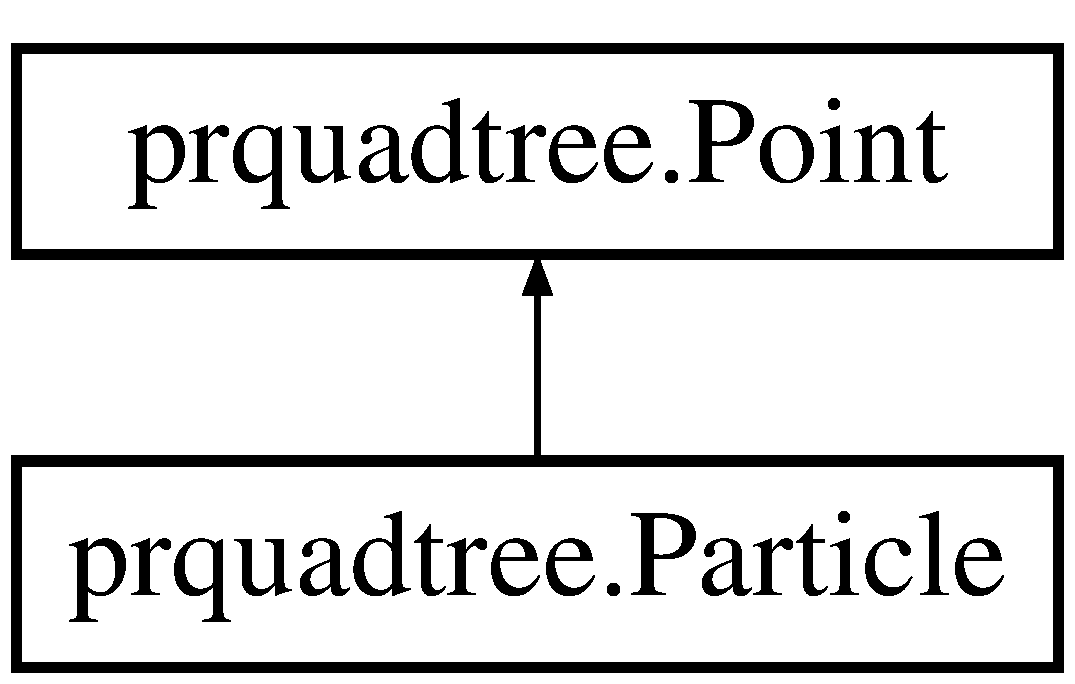
\includegraphics[height=2.000000cm]{classprquadtree_1_1Point}
\end{center}
\end{figure}
\subsection*{Public Member Functions}
\begin{DoxyCompactItemize}
\item 
def \hyperlink{classprquadtree_1_1Point_a1179022b24fec8ea7a8e0a7e9e7f664d}{\+\_\+\+\_\+init\+\_\+\+\_\+} (self, \hyperlink{classprquadtree_1_1Point_a769eeb814487b26593281a720cc43813}{x}, \hyperlink{classprquadtree_1_1Point_acc50fd274155e9a89996263a7e9f20db}{y})
\begin{DoxyCompactList}\small\item\em Constructs a coordinate \hyperlink{classprquadtree_1_1Point}{Point}. \end{DoxyCompactList}\item 
def \hyperlink{classprquadtree_1_1Point_ad33b3a05f6dce4daea0b307a42aa2453}{\+\_\+\+\_\+str\+\_\+\+\_\+} (self)
\begin{DoxyCompactList}\small\item\em Overwritting the default to string method of the \hyperlink{classprquadtree_1_1Point}{Point} class. \end{DoxyCompactList}\item 
def \hyperlink{classprquadtree_1_1Point_a8a9a5215cda0279f6958a0b55b4bc11d}{\+\_\+\+\_\+repr\+\_\+\+\_\+} (self)
\begin{DoxyCompactList}\small\item\em Needed for printing via \textquotesingle{}print\textquotesingle{}. \end{DoxyCompactList}\end{DoxyCompactItemize}
\subsection*{Public Attributes}
\begin{DoxyCompactItemize}
\item 
\hyperlink{classprquadtree_1_1Point_a769eeb814487b26593281a720cc43813}{x}
\item 
\hyperlink{classprquadtree_1_1Point_acc50fd274155e9a89996263a7e9f20db}{y}
\end{DoxyCompactItemize}


\subsection{Detailed Description}
Represents an (x,y) coordinate point on a grid. 



\subsection{Constructor \& Destructor Documentation}
\index{prquadtree\+::\+Point@{prquadtree\+::\+Point}!\+\_\+\+\_\+init\+\_\+\+\_\+@{\+\_\+\+\_\+init\+\_\+\+\_\+}}
\index{\+\_\+\+\_\+init\+\_\+\+\_\+@{\+\_\+\+\_\+init\+\_\+\+\_\+}!prquadtree\+::\+Point@{prquadtree\+::\+Point}}
\subsubsection[{\+\_\+\+\_\+init\+\_\+\+\_\+}]{\setlength{\rightskip}{0pt plus 5cm}def prquadtree.\+Point.\+\_\+\+\_\+init\+\_\+\+\_\+ (
\begin{DoxyParamCaption}
\item[{}]{self, }
\item[{}]{x, }
\item[{}]{y}
\end{DoxyParamCaption}
)}\label{classprquadtree_1_1Point_a1179022b24fec8ea7a8e0a7e9e7f664d}


Constructs a coordinate \hyperlink{classprquadtree_1_1Point}{Point}. 


\begin{DoxyParams}{Parameters}
{\em x} & float/int x-\/position \\
\hline
{\em y} & float/int y-\/position \\
\hline
\end{DoxyParams}


\subsection{Member Function Documentation}
\index{prquadtree\+::\+Point@{prquadtree\+::\+Point}!\+\_\+\+\_\+repr\+\_\+\+\_\+@{\+\_\+\+\_\+repr\+\_\+\+\_\+}}
\index{\+\_\+\+\_\+repr\+\_\+\+\_\+@{\+\_\+\+\_\+repr\+\_\+\+\_\+}!prquadtree\+::\+Point@{prquadtree\+::\+Point}}
\subsubsection[{\+\_\+\+\_\+repr\+\_\+\+\_\+}]{\setlength{\rightskip}{0pt plus 5cm}def prquadtree.\+Point.\+\_\+\+\_\+repr\+\_\+\+\_\+ (
\begin{DoxyParamCaption}
\item[{}]{self}
\end{DoxyParamCaption}
)}\label{classprquadtree_1_1Point_a8a9a5215cda0279f6958a0b55b4bc11d}


Needed for printing via \textquotesingle{}print\textquotesingle{}. 

\index{prquadtree\+::\+Point@{prquadtree\+::\+Point}!\+\_\+\+\_\+str\+\_\+\+\_\+@{\+\_\+\+\_\+str\+\_\+\+\_\+}}
\index{\+\_\+\+\_\+str\+\_\+\+\_\+@{\+\_\+\+\_\+str\+\_\+\+\_\+}!prquadtree\+::\+Point@{prquadtree\+::\+Point}}
\subsubsection[{\+\_\+\+\_\+str\+\_\+\+\_\+}]{\setlength{\rightskip}{0pt plus 5cm}def prquadtree.\+Point.\+\_\+\+\_\+str\+\_\+\+\_\+ (
\begin{DoxyParamCaption}
\item[{}]{self}
\end{DoxyParamCaption}
)}\label{classprquadtree_1_1Point_ad33b3a05f6dce4daea0b307a42aa2453}


Overwritting the default to string method of the \hyperlink{classprquadtree_1_1Point}{Point} class. 

\begin{DoxyReturn}{Returns}
String representation of \hyperlink{classprquadtree_1_1Point}{Point} 
\end{DoxyReturn}


\subsection{Member Data Documentation}
\index{prquadtree\+::\+Point@{prquadtree\+::\+Point}!x@{x}}
\index{x@{x}!prquadtree\+::\+Point@{prquadtree\+::\+Point}}
\subsubsection[{x}]{\setlength{\rightskip}{0pt plus 5cm}prquadtree.\+Point.\+x}\label{classprquadtree_1_1Point_a769eeb814487b26593281a720cc43813}
\index{prquadtree\+::\+Point@{prquadtree\+::\+Point}!y@{y}}
\index{y@{y}!prquadtree\+::\+Point@{prquadtree\+::\+Point}}
\subsubsection[{y}]{\setlength{\rightskip}{0pt plus 5cm}prquadtree.\+Point.\+y}\label{classprquadtree_1_1Point_acc50fd274155e9a89996263a7e9f20db}


The documentation for this class was generated from the following file\+:\begin{DoxyCompactItemize}
\item 
\hyperlink{prquadtree_8py}{prquadtree.\+py}\end{DoxyCompactItemize}

\hypertarget{classprquadtree_1_1PRQuadTree}{}\section{prquadtree.\+P\+R\+Quad\+Tree Class Reference}
\label{classprquadtree_1_1PRQuadTree}\index{prquadtree.\+P\+R\+Quad\+Tree@{prquadtree.\+P\+R\+Quad\+Tree}}
\subsection*{Public Member Functions}
\begin{DoxyCompactItemize}
\item 
def \hyperlink{classprquadtree_1_1PRQuadTree_a56de30271f808d21281b790a19448aab}{\+\_\+\+\_\+init\+\_\+\+\_\+} (self, \hyperlink{classprquadtree_1_1PRQuadTree_a2f1d8e21568aa0467a7dabedb50e3593}{box})
\item 
def \hyperlink{classprquadtree_1_1PRQuadTree_ab9ca8c1d94c56c72f47dabd2f90b7754}{insert} (self, point)
\item 
def \hyperlink{classprquadtree_1_1PRQuadTree_ab145cd20b246f04ddcd53ae9618b5479}{query\+\_\+range} (self, rng)
\item 
def \hyperlink{classprquadtree_1_1PRQuadTree_a578891ac618a6770184fc1c02f426b45}{query\+\_\+k\+\_\+nearest} (self, point, k)
\item 
def \hyperlink{classprquadtree_1_1PRQuadTree_a0d43d9d2ebe765b6690067c1d8bc5a8a}{print\+\_\+all\+\_\+points} (self, root)
\item 
def \hyperlink{classprquadtree_1_1PRQuadTree_a2f9dd431836575327c97cd3fb5426adb}{\+\_\+\+\_\+str\+\_\+\+\_\+} (self)
\end{DoxyCompactItemize}
\subsection*{Static Public Member Functions}
\begin{DoxyCompactItemize}
\item 
def \hyperlink{classprquadtree_1_1PRQuadTree_a5dd006b80f1697585a10722fba06e9ba}{size} (prtree)
\end{DoxyCompactItemize}
\subsection*{Public Attributes}
\begin{DoxyCompactItemize}
\item 
\hyperlink{classprquadtree_1_1PRQuadTree_a2f1d8e21568aa0467a7dabedb50e3593}{box}
\item 
\hyperlink{classprquadtree_1_1PRQuadTree_a6534693edb5dd5450859c5b4b0773936}{points}
\item 
\hyperlink{classprquadtree_1_1PRQuadTree_a6d0f1330cc70f704f8153fd1f386b9c3}{nw}
\item 
\hyperlink{classprquadtree_1_1PRQuadTree_acf96c88788ee32d03032c490b9a90f68}{ne}
\item 
\hyperlink{classprquadtree_1_1PRQuadTree_aee59816ff69872d39d406a103dd2e2f8}{sw}
\item 
\hyperlink{classprquadtree_1_1PRQuadTree_acf5a1f668e9962b03120856564e0a3b0}{se}
\end{DoxyCompactItemize}
\subsection*{Static Public Attributes}
\begin{DoxyCompactItemize}
\item 
int \hyperlink{classprquadtree_1_1PRQuadTree_a8a1b023159e61d011e1c1c94f3534a87}{Q\+T\+\_\+\+N\+O\+D\+E\+\_\+\+C\+A\+P\+A\+C\+I\+T\+Y} = 20
\end{DoxyCompactItemize}


\subsection{Detailed Description}
\begin{DoxyVerb}Class representing a Point Range Quadtree.
\end{DoxyVerb}
 

\subsection{Constructor \& Destructor Documentation}
\hypertarget{classprquadtree_1_1PRQuadTree_a56de30271f808d21281b790a19448aab}{}\index{prquadtree\+::\+P\+R\+Quad\+Tree@{prquadtree\+::\+P\+R\+Quad\+Tree}!\+\_\+\+\_\+init\+\_\+\+\_\+@{\+\_\+\+\_\+init\+\_\+\+\_\+}}
\index{\+\_\+\+\_\+init\+\_\+\+\_\+@{\+\_\+\+\_\+init\+\_\+\+\_\+}!prquadtree\+::\+P\+R\+Quad\+Tree@{prquadtree\+::\+P\+R\+Quad\+Tree}}
\subsubsection[{\+\_\+\+\_\+init\+\_\+\+\_\+}]{\setlength{\rightskip}{0pt plus 5cm}def prquadtree.\+P\+R\+Quad\+Tree.\+\_\+\+\_\+init\+\_\+\+\_\+ (
\begin{DoxyParamCaption}
\item[{}]{self, }
\item[{}]{box}
\end{DoxyParamCaption}
)}\label{classprquadtree_1_1PRQuadTree_a56de30271f808d21281b790a19448aab}
\begin{DoxyVerb}Constructs a PR Quadtree given an initial square.

Args:
    box: a Box representing initial square
\end{DoxyVerb}
 

\subsection{Member Function Documentation}
\hypertarget{classprquadtree_1_1PRQuadTree_a2f9dd431836575327c97cd3fb5426adb}{}\index{prquadtree\+::\+P\+R\+Quad\+Tree@{prquadtree\+::\+P\+R\+Quad\+Tree}!\+\_\+\+\_\+str\+\_\+\+\_\+@{\+\_\+\+\_\+str\+\_\+\+\_\+}}
\index{\+\_\+\+\_\+str\+\_\+\+\_\+@{\+\_\+\+\_\+str\+\_\+\+\_\+}!prquadtree\+::\+P\+R\+Quad\+Tree@{prquadtree\+::\+P\+R\+Quad\+Tree}}
\subsubsection[{\+\_\+\+\_\+str\+\_\+\+\_\+}]{\setlength{\rightskip}{0pt plus 5cm}def prquadtree.\+P\+R\+Quad\+Tree.\+\_\+\+\_\+str\+\_\+\+\_\+ (
\begin{DoxyParamCaption}
\item[{}]{self}
\end{DoxyParamCaption}
)}\label{classprquadtree_1_1PRQuadTree_a2f9dd431836575327c97cd3fb5426adb}
\begin{DoxyVerb}Prints the points of the nw,ne,sw,se blocks of the
given PRQuadTree node.

Returns:
    A string of points in the blocks
\end{DoxyVerb}
 \hypertarget{classprquadtree_1_1PRQuadTree_ab9ca8c1d94c56c72f47dabd2f90b7754}{}\index{prquadtree\+::\+P\+R\+Quad\+Tree@{prquadtree\+::\+P\+R\+Quad\+Tree}!insert@{insert}}
\index{insert@{insert}!prquadtree\+::\+P\+R\+Quad\+Tree@{prquadtree\+::\+P\+R\+Quad\+Tree}}
\subsubsection[{insert}]{\setlength{\rightskip}{0pt plus 5cm}def prquadtree.\+P\+R\+Quad\+Tree.\+insert (
\begin{DoxyParamCaption}
\item[{}]{self, }
\item[{}]{point}
\end{DoxyParamCaption}
)}\label{classprquadtree_1_1PRQuadTree_ab9ca8c1d94c56c72f47dabd2f90b7754}
\begin{DoxyVerb}Inserts a point into the PRQuadtree.

Args:
    point: An instance of Point

Returns:
    A boolean returning true on success, false on failure.
\end{DoxyVerb}
 \hypertarget{classprquadtree_1_1PRQuadTree_a0d43d9d2ebe765b6690067c1d8bc5a8a}{}\index{prquadtree\+::\+P\+R\+Quad\+Tree@{prquadtree\+::\+P\+R\+Quad\+Tree}!print\+\_\+all\+\_\+points@{print\+\_\+all\+\_\+points}}
\index{print\+\_\+all\+\_\+points@{print\+\_\+all\+\_\+points}!prquadtree\+::\+P\+R\+Quad\+Tree@{prquadtree\+::\+P\+R\+Quad\+Tree}}
\subsubsection[{print\+\_\+all\+\_\+points}]{\setlength{\rightskip}{0pt plus 5cm}def prquadtree.\+P\+R\+Quad\+Tree.\+print\+\_\+all\+\_\+points (
\begin{DoxyParamCaption}
\item[{}]{self, }
\item[{}]{root}
\end{DoxyParamCaption}
)}\label{classprquadtree_1_1PRQuadTree_a0d43d9d2ebe765b6690067c1d8bc5a8a}
\begin{DoxyVerb}Prints all points stored in the PRQuadtree.

Args:
    root: start point, or the root of the Quadtree

Returns:
    out: a string with coordinates
\end{DoxyVerb}
 \hypertarget{classprquadtree_1_1PRQuadTree_a578891ac618a6770184fc1c02f426b45}{}\index{prquadtree\+::\+P\+R\+Quad\+Tree@{prquadtree\+::\+P\+R\+Quad\+Tree}!query\+\_\+k\+\_\+nearest@{query\+\_\+k\+\_\+nearest}}
\index{query\+\_\+k\+\_\+nearest@{query\+\_\+k\+\_\+nearest}!prquadtree\+::\+P\+R\+Quad\+Tree@{prquadtree\+::\+P\+R\+Quad\+Tree}}
\subsubsection[{query\+\_\+k\+\_\+nearest}]{\setlength{\rightskip}{0pt plus 5cm}def prquadtree.\+P\+R\+Quad\+Tree.\+query\+\_\+k\+\_\+nearest (
\begin{DoxyParamCaption}
\item[{}]{self, }
\item[{}]{point, }
\item[{}]{k}
\end{DoxyParamCaption}
)}\label{classprquadtree_1_1PRQuadTree_a578891ac618a6770184fc1c02f426b45}
\begin{DoxyVerb}Returns k points closest to the provided point.

Args:
    point: a Point from which to search for other points.
    k: number of closest points to return

Returns:
    A list of k closest points
\end{DoxyVerb}
 \hypertarget{classprquadtree_1_1PRQuadTree_ab145cd20b246f04ddcd53ae9618b5479}{}\index{prquadtree\+::\+P\+R\+Quad\+Tree@{prquadtree\+::\+P\+R\+Quad\+Tree}!query\+\_\+range@{query\+\_\+range}}
\index{query\+\_\+range@{query\+\_\+range}!prquadtree\+::\+P\+R\+Quad\+Tree@{prquadtree\+::\+P\+R\+Quad\+Tree}}
\subsubsection[{query\+\_\+range}]{\setlength{\rightskip}{0pt plus 5cm}def prquadtree.\+P\+R\+Quad\+Tree.\+query\+\_\+range (
\begin{DoxyParamCaption}
\item[{}]{self, }
\item[{}]{rng}
\end{DoxyParamCaption}
)}\label{classprquadtree_1_1PRQuadTree_ab145cd20b246f04ddcd53ae9618b5479}
\begin{DoxyVerb}Returns the points in the provided range.

Args:
    rng: a Box range from which to retrieve points

Returns:
    A list of points within the provided range
\end{DoxyVerb}
 \hypertarget{classprquadtree_1_1PRQuadTree_a5dd006b80f1697585a10722fba06e9ba}{}\index{prquadtree\+::\+P\+R\+Quad\+Tree@{prquadtree\+::\+P\+R\+Quad\+Tree}!size@{size}}
\index{size@{size}!prquadtree\+::\+P\+R\+Quad\+Tree@{prquadtree\+::\+P\+R\+Quad\+Tree}}
\subsubsection[{size}]{\setlength{\rightskip}{0pt plus 5cm}def prquadtree.\+P\+R\+Quad\+Tree.\+size (
\begin{DoxyParamCaption}
\item[{}]{prtree}
\end{DoxyParamCaption}
)\hspace{0.3cm}{\ttfamily [static]}}\label{classprquadtree_1_1PRQuadTree_a5dd006b80f1697585a10722fba06e9ba}
\begin{DoxyVerb}Static method that determines the size of the given tree.
Keeping an insertion count in the client code would be
preferred to this due to heavy recursion.

Args:
    prtree: instance of PRQuadTree

Returns:
    An integer representing the number of points in the given tree.
\end{DoxyVerb}
 

\subsection{Member Data Documentation}
\hypertarget{classprquadtree_1_1PRQuadTree_a2f1d8e21568aa0467a7dabedb50e3593}{}\index{prquadtree\+::\+P\+R\+Quad\+Tree@{prquadtree\+::\+P\+R\+Quad\+Tree}!box@{box}}
\index{box@{box}!prquadtree\+::\+P\+R\+Quad\+Tree@{prquadtree\+::\+P\+R\+Quad\+Tree}}
\subsubsection[{box}]{\setlength{\rightskip}{0pt plus 5cm}prquadtree.\+P\+R\+Quad\+Tree.\+box}\label{classprquadtree_1_1PRQuadTree_a2f1d8e21568aa0467a7dabedb50e3593}
\hypertarget{classprquadtree_1_1PRQuadTree_acf96c88788ee32d03032c490b9a90f68}{}\index{prquadtree\+::\+P\+R\+Quad\+Tree@{prquadtree\+::\+P\+R\+Quad\+Tree}!ne@{ne}}
\index{ne@{ne}!prquadtree\+::\+P\+R\+Quad\+Tree@{prquadtree\+::\+P\+R\+Quad\+Tree}}
\subsubsection[{ne}]{\setlength{\rightskip}{0pt plus 5cm}prquadtree.\+P\+R\+Quad\+Tree.\+ne}\label{classprquadtree_1_1PRQuadTree_acf96c88788ee32d03032c490b9a90f68}
\hypertarget{classprquadtree_1_1PRQuadTree_a6d0f1330cc70f704f8153fd1f386b9c3}{}\index{prquadtree\+::\+P\+R\+Quad\+Tree@{prquadtree\+::\+P\+R\+Quad\+Tree}!nw@{nw}}
\index{nw@{nw}!prquadtree\+::\+P\+R\+Quad\+Tree@{prquadtree\+::\+P\+R\+Quad\+Tree}}
\subsubsection[{nw}]{\setlength{\rightskip}{0pt plus 5cm}prquadtree.\+P\+R\+Quad\+Tree.\+nw}\label{classprquadtree_1_1PRQuadTree_a6d0f1330cc70f704f8153fd1f386b9c3}
\hypertarget{classprquadtree_1_1PRQuadTree_a6534693edb5dd5450859c5b4b0773936}{}\index{prquadtree\+::\+P\+R\+Quad\+Tree@{prquadtree\+::\+P\+R\+Quad\+Tree}!points@{points}}
\index{points@{points}!prquadtree\+::\+P\+R\+Quad\+Tree@{prquadtree\+::\+P\+R\+Quad\+Tree}}
\subsubsection[{points}]{\setlength{\rightskip}{0pt plus 5cm}prquadtree.\+P\+R\+Quad\+Tree.\+points}\label{classprquadtree_1_1PRQuadTree_a6534693edb5dd5450859c5b4b0773936}
\hypertarget{classprquadtree_1_1PRQuadTree_a8a1b023159e61d011e1c1c94f3534a87}{}\index{prquadtree\+::\+P\+R\+Quad\+Tree@{prquadtree\+::\+P\+R\+Quad\+Tree}!Q\+T\+\_\+\+N\+O\+D\+E\+\_\+\+C\+A\+P\+A\+C\+I\+T\+Y@{Q\+T\+\_\+\+N\+O\+D\+E\+\_\+\+C\+A\+P\+A\+C\+I\+T\+Y}}
\index{Q\+T\+\_\+\+N\+O\+D\+E\+\_\+\+C\+A\+P\+A\+C\+I\+T\+Y@{Q\+T\+\_\+\+N\+O\+D\+E\+\_\+\+C\+A\+P\+A\+C\+I\+T\+Y}!prquadtree\+::\+P\+R\+Quad\+Tree@{prquadtree\+::\+P\+R\+Quad\+Tree}}
\subsubsection[{Q\+T\+\_\+\+N\+O\+D\+E\+\_\+\+C\+A\+P\+A\+C\+I\+T\+Y}]{\setlength{\rightskip}{0pt plus 5cm}int prquadtree.\+P\+R\+Quad\+Tree.\+Q\+T\+\_\+\+N\+O\+D\+E\+\_\+\+C\+A\+P\+A\+C\+I\+T\+Y = 20\hspace{0.3cm}{\ttfamily [static]}}\label{classprquadtree_1_1PRQuadTree_a8a1b023159e61d011e1c1c94f3534a87}
\hypertarget{classprquadtree_1_1PRQuadTree_acf5a1f668e9962b03120856564e0a3b0}{}\index{prquadtree\+::\+P\+R\+Quad\+Tree@{prquadtree\+::\+P\+R\+Quad\+Tree}!se@{se}}
\index{se@{se}!prquadtree\+::\+P\+R\+Quad\+Tree@{prquadtree\+::\+P\+R\+Quad\+Tree}}
\subsubsection[{se}]{\setlength{\rightskip}{0pt plus 5cm}prquadtree.\+P\+R\+Quad\+Tree.\+se}\label{classprquadtree_1_1PRQuadTree_acf5a1f668e9962b03120856564e0a3b0}
\hypertarget{classprquadtree_1_1PRQuadTree_aee59816ff69872d39d406a103dd2e2f8}{}\index{prquadtree\+::\+P\+R\+Quad\+Tree@{prquadtree\+::\+P\+R\+Quad\+Tree}!sw@{sw}}
\index{sw@{sw}!prquadtree\+::\+P\+R\+Quad\+Tree@{prquadtree\+::\+P\+R\+Quad\+Tree}}
\subsubsection[{sw}]{\setlength{\rightskip}{0pt plus 5cm}prquadtree.\+P\+R\+Quad\+Tree.\+sw}\label{classprquadtree_1_1PRQuadTree_aee59816ff69872d39d406a103dd2e2f8}


The documentation for this class was generated from the following file\+:\begin{DoxyCompactItemize}
\item 
\hyperlink{prquadtree_8py}{prquadtree.\+py}\end{DoxyCompactItemize}

\section{prquadtree\+\_\+test.\+Test\+Box Class Reference}
\label{classprquadtree__test_1_1TestBox}\index{prquadtree\+\_\+test.\+Test\+Box@{prquadtree\+\_\+test.\+Test\+Box}}
Inheritance diagram for prquadtree\+\_\+test.\+Test\+Box\+:\begin{figure}[H]
\begin{center}
\leavevmode
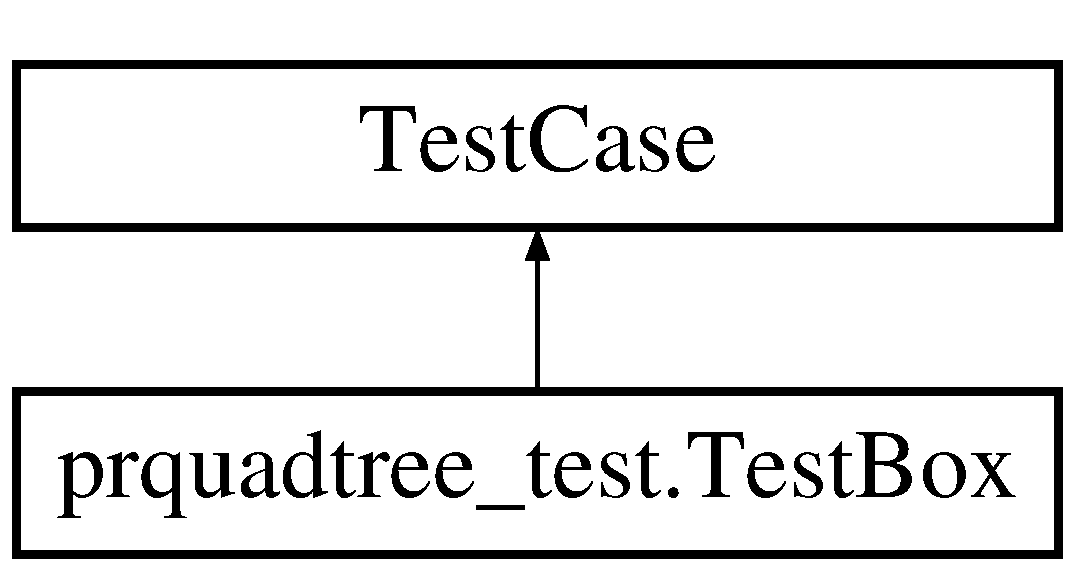
\includegraphics[height=2.000000cm]{classprquadtree__test_1_1TestBox}
\end{center}
\end{figure}
\subsection*{Public Member Functions}
\begin{DoxyCompactItemize}
\item 
def \hyperlink{classprquadtree__test_1_1TestBox_a58d746adb6903ff58eaf60bcaa08f4d4}{test\+\_\+box\+\_\+insert} (self)
\item 
def \hyperlink{classprquadtree__test_1_1TestBox_a059049f736a1ff093f4e0b3e5ed67f00}{test\+\_\+box\+\_\+contains} (self)
\end{DoxyCompactItemize}


\subsection{Member Function Documentation}
\index{prquadtree\+\_\+test\+::\+Test\+Box@{prquadtree\+\_\+test\+::\+Test\+Box}!test\+\_\+box\+\_\+contains@{test\+\_\+box\+\_\+contains}}
\index{test\+\_\+box\+\_\+contains@{test\+\_\+box\+\_\+contains}!prquadtree\+\_\+test\+::\+Test\+Box@{prquadtree\+\_\+test\+::\+Test\+Box}}
\subsubsection[{test\+\_\+box\+\_\+contains}]{\setlength{\rightskip}{0pt plus 5cm}def prquadtree\+\_\+test.\+Test\+Box.\+test\+\_\+box\+\_\+contains (
\begin{DoxyParamCaption}
\item[{}]{self}
\end{DoxyParamCaption}
)}\label{classprquadtree__test_1_1TestBox_a059049f736a1ff093f4e0b3e5ed67f00}
\index{prquadtree\+\_\+test\+::\+Test\+Box@{prquadtree\+\_\+test\+::\+Test\+Box}!test\+\_\+box\+\_\+insert@{test\+\_\+box\+\_\+insert}}
\index{test\+\_\+box\+\_\+insert@{test\+\_\+box\+\_\+insert}!prquadtree\+\_\+test\+::\+Test\+Box@{prquadtree\+\_\+test\+::\+Test\+Box}}
\subsubsection[{test\+\_\+box\+\_\+insert}]{\setlength{\rightskip}{0pt plus 5cm}def prquadtree\+\_\+test.\+Test\+Box.\+test\+\_\+box\+\_\+insert (
\begin{DoxyParamCaption}
\item[{}]{self}
\end{DoxyParamCaption}
)}\label{classprquadtree__test_1_1TestBox_a58d746adb6903ff58eaf60bcaa08f4d4}


The documentation for this class was generated from the following file\+:\begin{DoxyCompactItemize}
\item 
\hyperlink{prquadtree__test_8py}{prquadtree\+\_\+test.\+py}\end{DoxyCompactItemize}

\hypertarget{classprquadtree__test_1_1TestParticle}{}\section{prquadtree\+\_\+test.\+Test\+Particle Class Reference}
\label{classprquadtree__test_1_1TestParticle}\index{prquadtree\+\_\+test.\+Test\+Particle@{prquadtree\+\_\+test.\+Test\+Particle}}
Inheritance diagram for prquadtree\+\_\+test.\+Test\+Particle\+:\begin{figure}[H]
\begin{center}
\leavevmode
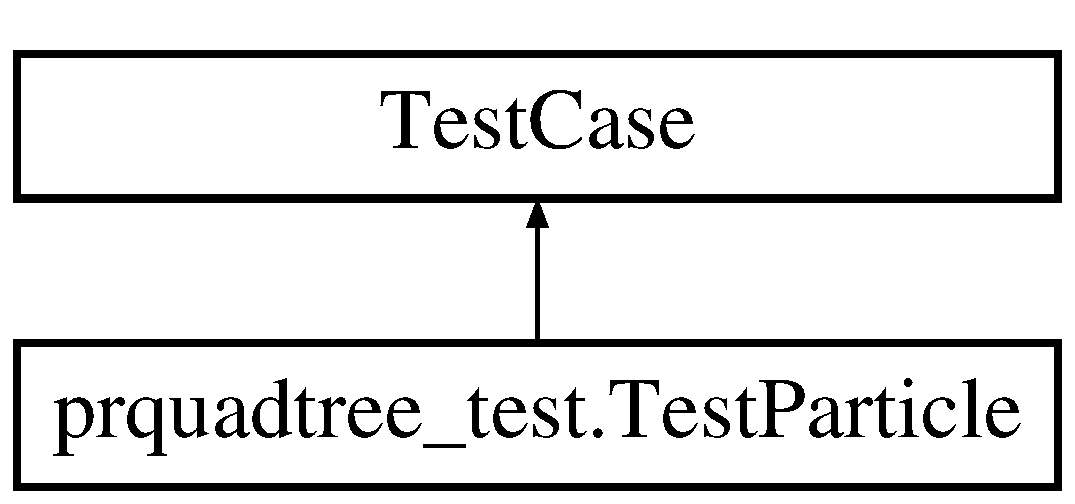
\includegraphics[height=2.000000cm]{classprquadtree__test_1_1TestParticle}
\end{center}
\end{figure}
\subsection*{Public Member Functions}
\begin{DoxyCompactItemize}
\item 
def \hyperlink{classprquadtree__test_1_1TestParticle_a64db3b2412e6487f7881ac2cf3e6a1a1}{test\+\_\+particle\+\_\+insert} (self)
\end{DoxyCompactItemize}


\subsection{Member Function Documentation}
\hypertarget{classprquadtree__test_1_1TestParticle_a64db3b2412e6487f7881ac2cf3e6a1a1}{}\index{prquadtree\+\_\+test\+::\+Test\+Particle@{prquadtree\+\_\+test\+::\+Test\+Particle}!test\+\_\+particle\+\_\+insert@{test\+\_\+particle\+\_\+insert}}
\index{test\+\_\+particle\+\_\+insert@{test\+\_\+particle\+\_\+insert}!prquadtree\+\_\+test\+::\+Test\+Particle@{prquadtree\+\_\+test\+::\+Test\+Particle}}
\subsubsection[{test\+\_\+particle\+\_\+insert}]{\setlength{\rightskip}{0pt plus 5cm}def prquadtree\+\_\+test.\+Test\+Particle.\+test\+\_\+particle\+\_\+insert (
\begin{DoxyParamCaption}
\item[{}]{self}
\end{DoxyParamCaption}
)}\label{classprquadtree__test_1_1TestParticle_a64db3b2412e6487f7881ac2cf3e6a1a1}


The documentation for this class was generated from the following file\+:\begin{DoxyCompactItemize}
\item 
\hyperlink{prquadtree__test_8py}{prquadtree\+\_\+test.\+py}\end{DoxyCompactItemize}

\hypertarget{classprquadtree__test_1_1TestPoint}{}\section{prquadtree\+\_\+test.\+Test\+Point Class Reference}
\label{classprquadtree__test_1_1TestPoint}\index{prquadtree\+\_\+test.\+Test\+Point@{prquadtree\+\_\+test.\+Test\+Point}}
Inheritance diagram for prquadtree\+\_\+test.\+Test\+Point\+:\begin{figure}[H]
\begin{center}
\leavevmode
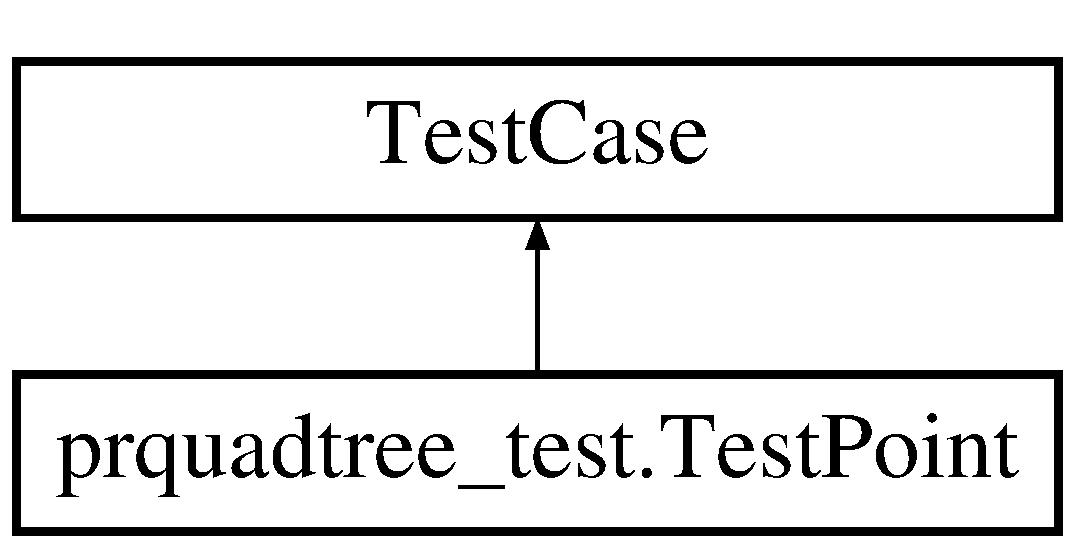
\includegraphics[height=2.000000cm]{classprquadtree__test_1_1TestPoint}
\end{center}
\end{figure}
\subsection*{Public Member Functions}
\begin{DoxyCompactItemize}
\item 
\hypertarget{classprquadtree__test_1_1TestPoint_a4d4ae74aeca57075dc73ceb7ca894077}{}def {\bfseries test\+\_\+point\+\_\+insert} (self)\label{classprquadtree__test_1_1TestPoint_a4d4ae74aeca57075dc73ceb7ca894077}

\end{DoxyCompactItemize}


The documentation for this class was generated from the following file\+:\begin{DoxyCompactItemize}
\item 
prquadtree\+\_\+test.\+py\end{DoxyCompactItemize}

\section{prquadtree\+\_\+test.\+Test\+Pr\+Quad\+Tree Class Reference}
\label{classprquadtree__test_1_1TestPrQuadTree}\index{prquadtree\+\_\+test.\+Test\+Pr\+Quad\+Tree@{prquadtree\+\_\+test.\+Test\+Pr\+Quad\+Tree}}
Inheritance diagram for prquadtree\+\_\+test.\+Test\+Pr\+Quad\+Tree\+:\begin{figure}[H]
\begin{center}
\leavevmode
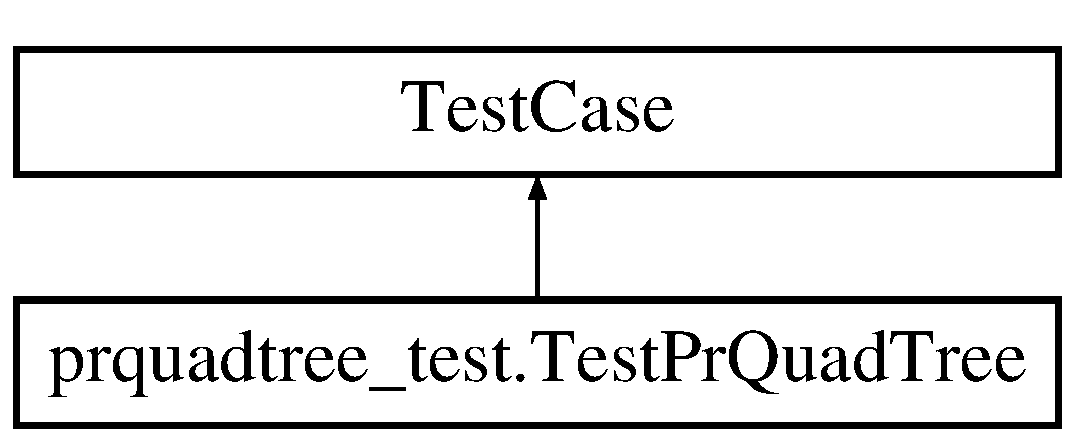
\includegraphics[height=2.000000cm]{classprquadtree__test_1_1TestPrQuadTree}
\end{center}
\end{figure}
\subsection*{Public Member Functions}
\begin{DoxyCompactItemize}
\item 
def \hyperlink{classprquadtree__test_1_1TestPrQuadTree_aa6b769cba631fb54c2576a35eb6f0681}{test\+\_\+insert} (self)
\item 
def \hyperlink{classprquadtree__test_1_1TestPrQuadTree_a6f5d504b57cae103ee89f7d347df9be4}{test\+\_\+nearby} (self)
\end{DoxyCompactItemize}


\subsection{Member Function Documentation}
\index{prquadtree\+\_\+test\+::\+Test\+Pr\+Quad\+Tree@{prquadtree\+\_\+test\+::\+Test\+Pr\+Quad\+Tree}!test\+\_\+insert@{test\+\_\+insert}}
\index{test\+\_\+insert@{test\+\_\+insert}!prquadtree\+\_\+test\+::\+Test\+Pr\+Quad\+Tree@{prquadtree\+\_\+test\+::\+Test\+Pr\+Quad\+Tree}}
\subsubsection[{test\+\_\+insert}]{\setlength{\rightskip}{0pt plus 5cm}def prquadtree\+\_\+test.\+Test\+Pr\+Quad\+Tree.\+test\+\_\+insert (
\begin{DoxyParamCaption}
\item[{}]{self}
\end{DoxyParamCaption}
)}\label{classprquadtree__test_1_1TestPrQuadTree_aa6b769cba631fb54c2576a35eb6f0681}
\index{prquadtree\+\_\+test\+::\+Test\+Pr\+Quad\+Tree@{prquadtree\+\_\+test\+::\+Test\+Pr\+Quad\+Tree}!test\+\_\+nearby@{test\+\_\+nearby}}
\index{test\+\_\+nearby@{test\+\_\+nearby}!prquadtree\+\_\+test\+::\+Test\+Pr\+Quad\+Tree@{prquadtree\+\_\+test\+::\+Test\+Pr\+Quad\+Tree}}
\subsubsection[{test\+\_\+nearby}]{\setlength{\rightskip}{0pt plus 5cm}def prquadtree\+\_\+test.\+Test\+Pr\+Quad\+Tree.\+test\+\_\+nearby (
\begin{DoxyParamCaption}
\item[{}]{self}
\end{DoxyParamCaption}
)}\label{classprquadtree__test_1_1TestPrQuadTree_a6f5d504b57cae103ee89f7d347df9be4}


The documentation for this class was generated from the following file\+:\begin{DoxyCompactItemize}
\item 
\hyperlink{prquadtree__test_8py}{prquadtree\+\_\+test.\+py}\end{DoxyCompactItemize}

\chapter{File Documentation}
\section{basket.\+py File Reference}
\label{basket_8py}\index{basket.\+py@{basket.\+py}}
\subsection*{Namespaces}
\begin{DoxyCompactItemize}
\item 
 \hyperlink{namespacebasket}{basket}
\end{DoxyCompactItemize}
\subsection*{Functions}
\begin{DoxyCompactItemize}
\item 
def \hyperlink{namespacebasket_a6244ca5fd7cf7706c81e45e270087d17}{basket.\+is\+\_\+basket\+\_\+middle} (img)
\begin{DoxyCompactList}\small\item\em Single entry function returning True/\+False if basket is in the middle of the screen. \end{DoxyCompactList}\item 
def \hyperlink{namespacebasket_a0cb50ef447247bf29a40cbdfcd275bc0}{basket.\+run\+\_\+middle} ()
\begin{DoxyCompactList}\small\item\em Runs continuously and prints if the best detected blob is in the middle. \end{DoxyCompactList}\item 
def \hyperlink{namespacebasket_a00c6a996da6d264c30c7b6c710cacddc}{basket.\+run}
\begin{DoxyCompactList}\small\item\em Runs continuously outlines best matched blob if it is in the middle. \end{DoxyCompactList}\end{DoxyCompactItemize}
\subsection*{Variables}
\begin{DoxyCompactItemize}
\item 
\hyperlink{namespacebasket_ae8e523df739d65470eb5eba16867f329}{basket.\+particle\+\_\+filter} = None
\item 
int \hyperlink{namespacebasket_a3c352b285b29250f904de2d4ad7fddaa}{basket.\+image\+\_\+half\+\_\+size} = -\/1
\item 
int \hyperlink{namespacebasket_a3d020674941ec4faf6734391ca082c40}{basket.\+save\+\_\+count} = 1
\item 
tuple \hyperlink{namespacebasket_aa3007fa12430ca814f5bf5890bb2fb0f}{basket.\+base\+\_\+filename} = datetime.\+now()
\end{DoxyCompactItemize}

\section{basket\+\_\+runner.\+py File Reference}
\label{basket__runner_8py}\index{basket\+\_\+runner.\+py@{basket\+\_\+runner.\+py}}
\subsection*{Namespaces}
\begin{DoxyCompactItemize}
\item 
 \hyperlink{namespacebasket__runner}{basket\+\_\+runner}
\end{DoxyCompactItemize}

\hypertarget{basket__test_8py}{}\section{basket\+\_\+test.\+py File Reference}
\label{basket__test_8py}\index{basket\+\_\+test.\+py@{basket\+\_\+test.\+py}}
\subsection*{Namespaces}
\begin{DoxyCompactItemize}
\item 
 \hyperlink{namespacebasket__test}{basket\+\_\+test}
\end{DoxyCompactItemize}
\subsection*{Functions}
\begin{DoxyCompactItemize}
\item 
def \hyperlink{namespacebasket__test_a6684d8ef9727f3f17d5177625d63f05b}{basket\+\_\+test.\+unit\+Test} (actual, expected, name)
\item 
def \hyperlink{namespacebasket__test_a6e9197dadee8f8fbbaef4c0015ba70d0}{basket\+\_\+test.\+basket\+Present} ()
\item 
def \hyperlink{namespacebasket__test_a02ba4e0e23e1661fbf650bfe5024dd5b}{basket\+\_\+test.\+basket\+Missing} ()
\end{DoxyCompactItemize}

\hypertarget{experiment_8py}{}\section{experiment.\+py File Reference}
\label{experiment_8py}\index{experiment.\+py@{experiment.\+py}}
\subsection*{Namespaces}
\begin{DoxyCompactItemize}
\item 
 \hyperlink{namespaceexperiment}{experiment}
\end{DoxyCompactItemize}
\subsection*{Functions}
\begin{DoxyCompactItemize}
\item 
def \hyperlink{namespaceexperiment_afd7cadc0db62c738ec5313cac9cd03e5}{experiment.\+experiment}
\item 
def \hyperlink{namespaceexperiment_aeac24644877a02c335d201812ba51625}{experiment.\+hard\+\_\+threshold} (img)
\item 
def \hyperlink{namespaceexperiment_afbfd0da7a229ea75fe6eda26e04a344a}{experiment.\+binary\+\_\+mask} (img)
\item 
def \hyperlink{namespaceexperiment_aad51fba16bbd81e9a968249d747958b3}{experiment.\+dilation\+\_\+and\+\_\+blur} (img)
\item 
def \hyperlink{namespaceexperiment_a26994eacbd1a8bf004fc3477c8164daf}{experiment.\+blobs\+\_\+by\+\_\+mask} (img)
\end{DoxyCompactItemize}

\section{image\+\_\+support.\+py File Reference}
\label{image__support_8py}\index{image\+\_\+support.\+py@{image\+\_\+support.\+py}}
\subsection*{Namespaces}
\begin{DoxyCompactItemize}
\item 
 \hyperlink{namespaceimage__support}{image\+\_\+support}
\end{DoxyCompactItemize}
\subsection*{Functions}
\begin{DoxyCompactItemize}
\item 
def \hyperlink{namespaceimage__support_a45e637a8685d23a453229102a4346327}{image\+\_\+support.\+external\+\_\+init\+\_\+particle\+\_\+filter} (img)
\item 
def \hyperlink{namespaceimage__support_aff0422e55f0d6119a012115570442c3f}{image\+\_\+support.\+image\+\_\+hue\+\_\+filter}
\item 
def \hyperlink{namespaceimage__support_aaa6d938c26b4ad5878e1bfb6870e749b}{image\+\_\+support.\+get\+\_\+hue\+\_\+blobs} (img)
\item 
def \hyperlink{namespaceimage__support_a0cebf9b300caec4b9e3f7725204f7f63}{image\+\_\+support.\+get\+\_\+best\+\_\+blob} (blobs, particle\+\_\+filter)
\item 
def \hyperlink{namespaceimage__support_ae76ebc019a04c735f46210bc29e55f76}{image\+\_\+support.\+is\+\_\+blob\+\_\+in\+\_\+middle\+\_\+helper} (img, blob)
\end{DoxyCompactItemize}
\subsection*{Variables}
\begin{DoxyCompactItemize}
\item 
int \hyperlink{namespaceimage__support_a1cfece0a81077dca0136b23884fb318d}{image\+\_\+support.\+bcolor} = 0
\end{DoxyCompactItemize}

\section{particlefilter.\+py File Reference}
\label{particlefilter_8py}\index{particlefilter.\+py@{particlefilter.\+py}}
\subsection*{Classes}
\begin{DoxyCompactItemize}
\item 
class \hyperlink{classparticlefilter_1_1ParticleFilter}{particlefilter.\+Particle\+Filter}
\end{DoxyCompactItemize}
\subsection*{Namespaces}
\begin{DoxyCompactItemize}
\item 
 \hyperlink{namespaceparticlefilter}{particlefilter}
\end{DoxyCompactItemize}

\section{prquadtree.\+py File Reference}
\label{prquadtree_8py}\index{prquadtree.\+py@{prquadtree.\+py}}
\subsection*{Classes}
\begin{DoxyCompactItemize}
\item 
class \hyperlink{classprquadtree_1_1Point}{prquadtree.\+Point}
\begin{DoxyCompactList}\small\item\em Represents an (x,y) coordinate point on a grid. \end{DoxyCompactList}\item 
class \hyperlink{classprquadtree_1_1Particle}{prquadtree.\+Particle}
\begin{DoxyCompactList}\small\item\em Represents particle point. \end{DoxyCompactList}\item 
class \hyperlink{classprquadtree_1_1Box}{prquadtree.\+Box}
\begin{DoxyCompactList}\small\item\em Class defining a square on the coordinate system via a center point and half of square width. \end{DoxyCompactList}\item 
class \hyperlink{classprquadtree_1_1PRQuadTree}{prquadtree.\+P\+R\+Quad\+Tree}
\begin{DoxyCompactList}\small\item\em Class representing a \hyperlink{classprquadtree_1_1Point}{Point} Range Quadtree. \end{DoxyCompactList}\end{DoxyCompactItemize}
\subsection*{Namespaces}
\begin{DoxyCompactItemize}
\item 
 \hyperlink{namespaceprquadtree}{prquadtree}
\end{DoxyCompactItemize}

\section{prquadtree\+\_\+test.\+py File Reference}
\label{prquadtree__test_8py}\index{prquadtree\+\_\+test.\+py@{prquadtree\+\_\+test.\+py}}
\subsection*{Classes}
\begin{DoxyCompactItemize}
\item 
class \hyperlink{classprquadtree__test_1_1TestPoint}{prquadtree\+\_\+test.\+Test\+Point}
\item 
class \hyperlink{classprquadtree__test_1_1TestParticle}{prquadtree\+\_\+test.\+Test\+Particle}
\item 
class \hyperlink{classprquadtree__test_1_1TestBox}{prquadtree\+\_\+test.\+Test\+Box}
\item 
class \hyperlink{classprquadtree__test_1_1TestPrQuadTree}{prquadtree\+\_\+test.\+Test\+Pr\+Quad\+Tree}
\end{DoxyCompactItemize}
\subsection*{Namespaces}
\begin{DoxyCompactItemize}
\item 
 \hyperlink{namespaceprquadtree__test}{prquadtree\+\_\+test}
\end{DoxyCompactItemize}

\section{prquadtree\+\_\+test\+\_\+example.\+py File Reference}
\label{prquadtree__test__example_8py}\index{prquadtree\+\_\+test\+\_\+example.\+py@{prquadtree\+\_\+test\+\_\+example.\+py}}
\subsection*{Namespaces}
\begin{DoxyCompactItemize}
\item 
 \hyperlink{namespaceprquadtree__test__example}{prquadtree\+\_\+test\+\_\+example}
\end{DoxyCompactItemize}
\subsection*{Variables}
\begin{DoxyCompactItemize}
\item 
tuple \hyperlink{namespaceprquadtree__test__example_a430c6e4c1960cb0326d40a60be817d65}{prquadtree\+\_\+test\+\_\+example.\+b} = Box(Point(5,5), 50)
\item 
tuple \hyperlink{namespaceprquadtree__test__example_a6c76891a5f566a70e8ab91c9946be5a2}{prquadtree\+\_\+test\+\_\+example.\+b2} = Box(Point(50,50), 50)
\item 
tuple \hyperlink{namespaceprquadtree__test__example_a92699a8bb92121b0ffdac66d511f3359}{prquadtree\+\_\+test\+\_\+example.\+qt} = P\+R\+Quad\+Tree(b2)
\item 
tuple \hyperlink{namespaceprquadtree__test__example_ab0091dbc0243fa027e0bc7025d8ea3ad}{prquadtree\+\_\+test\+\_\+example.\+pt} = Point(2,2)
\item 
tuple \hyperlink{namespaceprquadtree__test__example_a2024920106d8770dc2cfa9da1e4fe410}{prquadtree\+\_\+test\+\_\+example.\+nearby} = qt.\+query\+\_\+k\+\_\+nearest(pt, 20)
\item 
int \hyperlink{namespaceprquadtree__test__example_a51f7199631c374c21ed3dada86cc3766}{prquadtree\+\_\+test\+\_\+example.\+c} = 1
\end{DoxyCompactItemize}

\hypertarget{tennis__ball_8py}{}\section{tennis\+\_\+ball.\+py File Reference}
\label{tennis__ball_8py}\index{tennis\+\_\+ball.\+py@{tennis\+\_\+ball.\+py}}
\subsection*{Namespaces}
\begin{DoxyCompactItemize}
\item 
 \hyperlink{namespacetennis__ball}{tennis\+\_\+ball}
\end{DoxyCompactItemize}
\subsection*{Functions}
\begin{DoxyCompactItemize}
\item 
def \hyperlink{namespacetennis__ball_a595850f165f1ae2c78218d580854bfda}{tennis\+\_\+ball.\+is\+\_\+ball\+\_\+middle} (img)
\item 
def \hyperlink{namespacetennis__ball_af2aced0030d28f7b0b98175dd3a3d97c}{tennis\+\_\+ball.\+run} ()
\end{DoxyCompactItemize}
\subsection*{Variables}
\begin{DoxyCompactItemize}
\item 
\hyperlink{namespacetennis__ball_aba3913b89ed8c5fae700b6dfbca98f05}{tennis\+\_\+ball.\+particle\+\_\+filter} = None
\end{DoxyCompactItemize}

\section{tennis\+\_\+ball\+\_\+runner.\+py File Reference}
\label{tennis__ball__runner_8py}\index{tennis\+\_\+ball\+\_\+runner.\+py@{tennis\+\_\+ball\+\_\+runner.\+py}}
\subsection*{Namespaces}
\begin{DoxyCompactItemize}
\item 
 \hyperlink{namespacetennis__ball__runner}{tennis\+\_\+ball\+\_\+runner}
\end{DoxyCompactItemize}

\section{tennis\+\_\+ball\+\_\+test.\+py File Reference}
\label{tennis__ball__test_8py}\index{tennis\+\_\+ball\+\_\+test.\+py@{tennis\+\_\+ball\+\_\+test.\+py}}
\subsection*{Namespaces}
\begin{DoxyCompactItemize}
\item 
 \hyperlink{namespacetennis__ball__test}{tennis\+\_\+ball\+\_\+test}
\end{DoxyCompactItemize}
\subsection*{Functions}
\begin{DoxyCompactItemize}
\item 
def \hyperlink{namespacetennis__ball__test_a377f9e4b2c183f3b84a826938e92b1d3}{tennis\+\_\+ball\+\_\+test.\+unit\+Test} (actual, expected, name)
\item 
def \hyperlink{namespacetennis__ball__test_ae38438bf59080ab5cb67dc008a0e05b5}{tennis\+\_\+ball\+\_\+test.\+ball\+Present} ()
\item 
def \hyperlink{namespacetennis__ball__test_a62d3502cccff6477767acdf8cf20caab}{tennis\+\_\+ball\+\_\+test.\+ball\+Missing} ()
\end{DoxyCompactItemize}

\hypertarget{visual_8h}{}\section{visual.\+h File Reference}
\label{visual_8h}\index{visual.\+h@{visual.\+h}}
\subsection*{Functions}
\begin{DoxyCompactItemize}
\item 
int \hyperlink{visual_8h_a67d84fc9e33637d003f6d92ad11684e7}{start\+\_\+visual} (void)
\item 
void \hyperlink{visual_8h_a5f11f954300b2bbd867500a13724ad09}{set\+\_\+objects} (object\+\_\+t $\ast$objs)
\item 
void \hyperlink{visual_8h_a1f0452966043876e4b97d6696547e9e1}{get\+\_\+objects} (object\+\_\+t $\ast$objs, point\+\_\+t $\ast$locations)
\item 
void \hyperlink{visual_8h_abc6a6c455959f4fb0fbd3cf0f46e7d40}{stop\+\_\+visual} (void)
\end{DoxyCompactItemize}


\subsection{Function Documentation}
\hypertarget{visual_8h_a1f0452966043876e4b97d6696547e9e1}{}\index{visual.\+h@{visual.\+h}!get\+\_\+objects@{get\+\_\+objects}}
\index{get\+\_\+objects@{get\+\_\+objects}!visual.\+h@{visual.\+h}}
\subsubsection[{get\+\_\+objects}]{\setlength{\rightskip}{0pt plus 5cm}void get\+\_\+objects (
\begin{DoxyParamCaption}
\item[{object\+\_\+t $\ast$}]{objs, }
\item[{point\+\_\+t $\ast$}]{locations}
\end{DoxyParamCaption}
)}\label{visual_8h_a1f0452966043876e4b97d6696547e9e1}
\hypertarget{visual_8h_a5f11f954300b2bbd867500a13724ad09}{}\index{visual.\+h@{visual.\+h}!set\+\_\+objects@{set\+\_\+objects}}
\index{set\+\_\+objects@{set\+\_\+objects}!visual.\+h@{visual.\+h}}
\subsubsection[{set\+\_\+objects}]{\setlength{\rightskip}{0pt plus 5cm}void set\+\_\+objects (
\begin{DoxyParamCaption}
\item[{object\+\_\+t $\ast$}]{objs}
\end{DoxyParamCaption}
)}\label{visual_8h_a5f11f954300b2bbd867500a13724ad09}
\hypertarget{visual_8h_a67d84fc9e33637d003f6d92ad11684e7}{}\index{visual.\+h@{visual.\+h}!start\+\_\+visual@{start\+\_\+visual}}
\index{start\+\_\+visual@{start\+\_\+visual}!visual.\+h@{visual.\+h}}
\subsubsection[{start\+\_\+visual}]{\setlength{\rightskip}{0pt plus 5cm}int start\+\_\+visual (
\begin{DoxyParamCaption}
\item[{void}]{}
\end{DoxyParamCaption}
)}\label{visual_8h_a67d84fc9e33637d003f6d92ad11684e7}
\hypertarget{visual_8h_abc6a6c455959f4fb0fbd3cf0f46e7d40}{}\index{visual.\+h@{visual.\+h}!stop\+\_\+visual@{stop\+\_\+visual}}
\index{stop\+\_\+visual@{stop\+\_\+visual}!visual.\+h@{visual.\+h}}
\subsubsection[{stop\+\_\+visual}]{\setlength{\rightskip}{0pt plus 5cm}void stop\+\_\+visual (
\begin{DoxyParamCaption}
\item[{void}]{}
\end{DoxyParamCaption}
)}\label{visual_8h_abc6a6c455959f4fb0fbd3cf0f46e7d40}

%--- End generated contents ---

% Index
\backmatter
\newpage
\phantomsection
\clearemptydoublepage
\addcontentsline{toc}{chapter}{Index}
\printindex

\end{document}
